%% abtex2-modelo-trabalho-academico.tex, v-1.7.1 laurocesar
%% Copyright 2012-2013 by abnTeX2 group at http://abntex2.googlecode.com/ 
%%
%% This work may be distributed and/or modified under the
%% conditions of the LaTeX Project Public License, either version 1.3
%% of this license or (at your option) any later version.
%% The latest version of this license is in
%%   http://www.latex-project.org/lppl.txt
%% and version 1.3 or later is part of all distributions of LaTeX
%% version 2005/12/01 or later.
%%
%% This work has the LPPL maintenance status `maintained'.
%% 
%% The Current Maintainer of this work is the abnTeX2 team, led
%% by Lauro César Araujo. Further information are available on 
%% http://abntex2.googlecode.com/
%%
%% This work consists of the files abntex2-modelo-trabalho-academico.tex,
%% abntex2-modelo-include-comandos and abntex2-modelo-references.bib
%%

% ------------------------------------------------------------------------
% ------------------------------------------------------------------------
% abnTeX2: Modelo de Trabalho Academico (tese de doutorado, dissertacao de
% mestrado e trabalhos monograficos em geral) em conformidade com 
% ABNT NBR 14724:2011: Informacao e documentacao - Trabalhos academicos -
% Apresentacao
% ------------------------------------------------------------------------
% ------------------------------------------------------------------------

\documentclass[
    article,
	% -- opções da classe memoir --
	12pt,				% tamanho da fonte
	openright,			% capítulos começam em pág ímpar (insere página vazia caso preciso)
	twoside,			% para impressão em verso e anverso. Oposto a oneside
	a4paper,			% tamanho do papel. 
	% -- opções da classe abntex2 --
	%chapter=TITLE,		% títulos de capítulos convertidos em letras maiúsculas
	%section=TITLE,		% títulos de seções convertidos em letras maiúsculas
	%subsection=TITLE,	% títulos de subseções convertidos em letras maiúsculas
	%subsubsection=TITLE,% títulos de subsubseções convertidos em letras maiúsculas
	% -- opções do pacote babel --
	english,			% idioma adicional para hifenização
% 	french,				% idioma adicional para hifenização
	spanish,			% idioma adicional para hifenização
	brazil,				% o último idioma é o principal do documento
	]{abntex2}


% ---
% PACOTES
% ---

% ---
% Pacotes fundamentais 
% ---

\usepackage[table,xcdraw]{xcolor}
\usepackage{cmap}				% Mapear caracteres especiais no PDF
\usepackage{lmodern}			% Usa a fonte Latin Modern			
\usepackage[T1]{fontenc}		% Selecao de codigos de fonte.
\usepackage[utf8]{inputenc}		% Codificacao do documento (conversão automática dos acentos)
\usepackage{lastpage}			% Usado pela Ficha catalográfica
\usepackage{indentfirst}		% Indenta o primeiro parágrafo de cada seção.
\usepackage{color}				% Controle das cores
\usepackage{graphicx}			% Inclusão de gráficos
\usepackage{amsmath}            % Equações matemáticas
% ---
\usepackage[authoryear,round,longnamesfirst]{natbib} %% citep e citet
\usepackage{natbib} %% citep e citet
% % \bibliographystyle{unsrtnat}
% \bibliographystyle{dinat}
% ---
% Pacotes adicionais, usados apenas no âmbito do Modelo Canônico do abnteX2
% ---
\usepackage{lipsum}				% para geração de dummy text
\usepackage{caption}
\usepackage{subcaption}
% ---
% Data em portugues
% \usepackage[portuguese]{babel}
% ---
% Pacotes de citações
% ---
\usepackage[brazilian,hyperpageref]{backref}	 % Paginas com as citações na bibl
% \usepackage[alf]{abntex2cite}	% Citações padrão ABNT

% Citacoes por natbib

\usepackage{natbib}

\usepackage{algorithm}% http://ctan.org/pkg/algorithms
\makeatletter
\renewcommand{\ALG@name}{Algoritmo}
\makeatother

\makeatletter
\renewcommand{\listalgorithmname}{Lista de \ALG@name s}
\makeatother

\usepackage[noend]{algpseudocode}% http://ctan.org/pkg/algorithmicx
\usepackage{lmodern}% http://ctan.org/pkg/lmodern
\bibliographystyle{humannat}
% \bibliographystyle{sbc-template}

% --- 
% CONFIGURAÇÕES DE PACOTES
% --- 

% ---
% Configurações do pacote backref
% Usado sem a opção hyperpageref de backref
\renewcommand{\backrefpagesname}{Citado na(s) página(s):~}
% Texto padrão antes do número das páginas
\renewcommand{\backref}{}
\newcommand{\mc}[1]{\mathcal{#1}}
% Define os textos da citação
\renewcommand*{\backrefalt}[4]{
	\ifcase #1 %
		Nenhuma citação no texto.%
	\or
		Citado na página #2.%
	\else
		Citado #1 vezes nas páginas #2.%
	\fi}%
% ---


% ---
% Informações de dados para CAPA e FOLHA DE ROSTO
% ---
\titulo{Combinando busca binária exata e busca aproximada em sistemas de complementação automática de consultas}
\autor{Rúben Jozafá Silva Belém}
\local{Brasil}
\data{2020}
\orientador{Prof. Dr. Edleno Silva de Moura}
% \coorientador{Equipe \abnTeX}
\instituicao{%
  Universidade Federal do Amazonas -- UFAM
  \par
  Instituto de Computação -- ICOMP
  \par
  Programa de Pós-Graduação em Informática -- PPGI}
\tipotrabalho{Qualificação (Mestrado)}
% O preambulo deve conter o tipo do trabalho, o objetivo, 
% o nome da instituição e a área de concentração 
\preambulo{Proposta de qualificação apresentada ao Instituto de Computação da Universidade Federal do Amazonas como requisito para obtenção da qualificação para mestrado em Informática.}
% ---


% ---
% Configurações de aparência do PDF final

% alterando o aspecto da cor azul
\definecolor{blue}{RGB}{41,5,195}

% informações do PDF
\makeatletter
\hypersetup{
     	%pagebackref=true,
		pdftitle={\@title}, 
		pdfauthor={\@author},
    	pdfsubject={\imprimirpreambulo},
	    pdfcreator={LaTeX with abnTeX2},
		pdfkeywords={abnt}{latex}{abntex}{abntex2}{trabalho acadêmico}, 
		colorlinks=true,       		% false: boxed links; true: colored links
    	linkcolor=blue,          	% color of internal links
    	citecolor=blue,        		% color of links to bibliography
    	filecolor=magenta,      		% color of file links
		urlcolor=blue,
		bookmarksdepth=4
}
\makeatother
% --- 

% --- 
% Espaçamentos entre linhas e parágrafos 
% --- 

% O tamanho do parágrafo é dado por:
\setlength{\parindent}{1.3cm}

% Controle do espaçamento entre um parágrafo e outro:
\setlength{\parskip}{0.2cm}  % tente também \onelineskip

% ---
% compila o indice
% ---
\makeindex
% ---

% ----
% Início do documento
% ----
\begin{document}

% Retira espaço extra obsoleto entre as frases.
\frenchspacing 

% ----------------------------------------------------------
% ELEMENTOS PRÉ-TEXTUAIS
% ----------------------------------------------------------
 \pretextual

% ---
% Capa
% ---
\imprimircapa
% ---

% ---
% Folha de rosto
% (o * indica que haverá a ficha bibliográfica)
% ---

\imprimirfolhaderosto* 

% ---

% ---
% Inserir a ficha bibliografica
% ---

% Isto é um exemplo de Ficha Catalográfica, ou ``Dados internacionais de
% catalogação-na-publicação''. Você pode utilizar este modelo como referência. 
% Porém, provavelmente a biblioteca da sua universidade lhe fornecerá um PDF
% com a ficha catalográfica definitiva após a defesa do trabalho. Quando estiver
% com o documento, salve-o como PDF no diretório do seu projeto e substitua todo
% o conteúdo de implementação deste arquivo pelo comando abaixo:
%
% \begin{fichacatalografica}
%     \includepdf{fig_ficha_catalografica.pdf}
% \end{fichacatalografica}


% \begin{fichacatalografica}
% 	\vspace*{\fill}					% Posição vertical
% 	\hrule							% Linha horizontal
% 	\begin{center}					% Minipage Centralizado
% 	\begin{minipage}[c]{12.5cm}		% Largura
	
% 	\imprimirautor
	
% 	\hspace{0.5cm} \imprimirtitulo  / \imprimirautor. --
% 	\imprimirlocal, \imprimirdata-
	
% 	\hspace{0.5cm} \pageref{LastPage} p. : il. (algumas color.) ; 30 cm.\\
	
% 	\hspace{0.5cm} \imprimirorientadorRotulo~\imprimirorientador\\
	
% 	\hspace{0.5cm}
% 	\parbox[t]{\textwidth}{\imprimirtipotrabalho~--~\imprimirinstituicao,
% 	\imprimirdata.}\\
	
% 	\hspace{0.5cm}
% 		1. Phrasal Terms.
% 		2. Query Terms.
% 		I. Edleno Silva de Moura.
% 		II. Universidade Federal do Amazonas.
% 		III. Instituto de Computação.
% 		IV. Aplicação de Informações Estatísticas na Busca por Phrasal Terms\\ 			
	
% 	\hspace{8.75cm} CDU 02:141:005.7\\
	
% 	\end{minipage}
% 	\end{center}
% 	\hrule
% \end{fichacatalografica}

% ---

% ---
% Inserir errata
% ---

% \begin{errata}
% Elemento opcional da \citeonline[4.2.1.2]{NBR14724:2011}. Exemplo:

% \vspace{\onelineskip}

% FERRIGNO, C. R. A. \textbf{Tratamento de neoplasias ósseas apendiculares com
% reimplantação de enxerto ósseo autólogo autoclavado associado ao plasma
% rico em plaquetas}: estudo crítico na cirurgia de preservação de membro em
% cães. 2011. 128 f. Tese (Livre-Docência) - Faculdade de Medicina Veterinária e
% Zootecnia, Universidade de São Paulo, São Paulo, 2011.

% \begin{table}[htb]
% \center
% \footnotesize
% \begin{tabular}{|p{1.4cm}|p{1cm}|p{3cm}|p{3cm}|}
%   \hline
%    \textbf{Folha} & \textbf{Linha}  & \textbf{Onde se lê}  & \textbf{Leia-se}  \\
%     \hline
%     1 & 10 & auto-conclavo & autoconclavo\\
%    \hline
% \end{tabular}
% \end{table}

% \end{errata}

% ---

% ---
% Inserir folha de aprovação
% ---

% Isto é um exemplo de Folha de aprovação, elemento obrigatório da NBR
% 14724/2011 (seção 4.2.1.3). Você pode utilizar este modelo até a aprovação
% do trabalho. Após isso, substitua todo o conteúdo deste arquivo por uma
% imagem da página assinada pela banca com o comando abaixo:

% \includepdf{folhadeaprovacao_final.pdf}



% \begin{folhadeaprovacao}

%   \begin{center}
%     {\ABNTEXchapterfont\large\imprimirautor}

%     \vspace*{\fill}\vspace*{\fill}
%     {\ABNTEXchapterfont\bfseries\Large\imprimirtitulo}
%     \vspace*{\fill}
    
%     \hspace{.45\textwidth}
%     \begin{minipage}{.5\textwidth}
%         \imprimirpreambulo
%     \end{minipage}%
%     \vspace*{\fill}
%   \end{center}
    
%   Trabalho aprovado. \imprimirlocal, \today:

%   \assinatura{\textbf{\imprimirorientador} \\ Orientador} 
% %   \assinatura{\textbf{Prof. Dr. Altigran S. da Silva} \\ Convidado 1}
% %   \assinatura{\textbf{Prof. Dr. Marco Antônio Pinho de Cristo} \\ Convidado 2}
%   %\assinatura{\textbf{Professor} \\ Convidado 3}
%   %\assinatura{\textbf{Professor} \\ Convidado 4}
      
%   \begin{center}
%     \vspace*{0.5cm}
%     {\large\imprimirlocal}
%     \par
%     {\large\imprimirdata}
%     \vspace*{1cm}
%   \end{center}
  
% \end{folhadeaprovacao}



% ---

% ---
% Dedicatória
% ---
% \begin{dedicatoria}
%    \vspace*{\fill}
%    \centering
%    \noindent
%    \textit{ Este trabalho é dedicado às crianças adultas que,\\
%    quando pequenas, sonharam em se tornar cientistas.} \vspace*{\fill}
% \end{dedicatoria}
% ---

% ---
% Agradecimentos
% ---
% \begin{agradecimentos}
% Os agradecimentos principais são direcionados à Gerald Weber, Miguel Frasson,
% Leslie H. Watter, Bruno Parente Lima, Flávio de Vasconcellos Corrêa, Otavio Real
% Salvador, Renato Machnievscz\footnote{Os nomes dos integrantes do primeiro
% projeto abn\TeX\ foram extraídos de
% \url{http://codigolivre.org.br/projects/abntex/}} e todos aqueles que
% contribuíram para que a produção de trabalhos acadêmicos conforme
% as normas ABNT com \LaTeX\ fosse possível.

% Agradecimentos especiais são direcionados ao Centro de Pesquisa em Arquitetura
% da Informação\footnote{\url{http://www.cpai.unb.br/}} da Universidade de
% Brasília (CPAI), ao grupo de usuários
% \emph{latex-br}\footnote{\url{http://groups.google.com/group/latex-br}} e aos
% novos voluntários do grupo
% \emph{\abnTeX}\footnote{\url{http://groups.google.com/group/abntex2} e
% \url{http://abntex2.googlecode.com/}}~que contribuíram e que ainda
% contribuirão para a evolução do \abnTeX.

% \end{agradecimentos}
% ---

% ---
% Epígrafe
% ---
% \begin{epigrafe}
%     \vspace*{\fill}
% 	\begin{flushright}
% 		\textit{``Não vos amoldeis às estruturas deste mundo, \\
% 		mas transformai-vos pela renovação da mente, \\
% 		a fim de distinguir qual é a vontade de Deus: \\
% 		o que é bom, o que Lhe é agradável, o que é perfeito.\\
% 		(Bíblia Sagrada, Romanos 12, 2)}
% 	\end{flushright}
% \end{epigrafe}
% ---

% ---
% RESUMOS
% ---

% resumo em português
\begin{resumo}
A forma tradicional de acesso aos dados com consultas por palavras-chave se dá por meio da utilização de texto completo, mas esse paradigma exige que o usuário possua uma noção sobre a estrutura do conteúdo do repositório de dados. Para reduzir o esforço necessário para a realização de consultas os motores de busca recentemente têm amplamente adotado a complementação automática de consultas, e além disso, uma vez que o usuário pode cometer erros de digitação, também têm tolerado tais erros. As soluções mais eficientes dos últimos anos são baseadas em índices de árvore \textit{Trie}, no entanto, esse tipo de solução pode utilizar grande quantidade de memória.
Este trabalho apresenta uma estrutura em dois níveis que utiliza índices de árvore \textit{Trie} no primeiro nível, e uma combinação de buscas sequencial e binária no segundo.
A estrutura apresentada foi capaz de atingir o objetivo de realizar busca reduzindo o consumo de memória, mas mantendo o desempenho similar ao uso da estrutura de busca em apenas um nível. 
 	
% \noindent
% \textbf{Palavras-chave}: Em desenvolvimento ...
 
\vspace{\onelineskip}
 

    
 \noindent
%  \textbf{Palavras-chaves}: Em desenvolvimento ...
\end{resumo}


% % % resumo em inglês
% \begin{resumo}[Abstract]
%  \begin{otherlanguage*}{english}
%   Em desenvolvimento...

%   \vspace{\onelineskip}
 
%   \noindent 
%   \textbf{Key-words}: Em desenvolvimento ...
%  \end{otherlanguage*}
% \end{resumo}

% resumo em francês 
% \begin{resumo}[Résumé]
%  \begin{otherlanguage*}{french}
%     Il s'agit d'un résumé en français.
 
%     \vspace{\onelineskip}
 
%     \noindent
%     \textbf{Mots-clés}: latex. abntex. publication de textes.
%  \end{otherlanguage*}
% \end{resumo}

% resumo em espanhol
% \begin{resumo}[Resumen]
%  \begin{otherlanguage*}{spanish}
%     Este es el resumen en español.
  
%     \vspace{\onelineskip}
 
%     \noindent
%     \textbf{Palabras clave}: latex. abntex. publicación de textos.
%  \end{otherlanguage*}
% \end{resumo}
% ---
\newpage
% ---
% inserir lista de ilustrações
% ---
\pdfbookmark[0]{\listfigurename}{lof}
\listoffigures*
\cleardoublepage
% ---

% ---
% inserir lista de tabelas
% ---
\pdfbookmark[0]{\listtablename}{lot}
\listoftables*
\cleardoublepage

\makeatletter
\renewcommand\numberline[1]{
    \leftskip -0.7em
    \rightskip 1.6em
    \parfillskip -\rightskip
    \parindent 0em
    \@tempdima 2.0em
    \vspace{0em} \advance\leftskip \@tempdima \null\nobreak\hskip -\leftskip
    Algoritmo \normalfont #1 – }
\makeatother
\listofalgorithms
\cleardoublepage

\makeatletter
\def\numberline#1{\hb@xt@\@tempdima{#1\hfil}}
\makeatother

% ---
% inserir lista de abreviaturas e siglas
% ---
% \begin{siglas}
%   \item[TF] Termo Frasal
%   \item[RI] Recuperação de Informação
%   \item[SVM] Support Vector Machine
%   \item[NP] Noun Phrase
%   \item[VP] Verb Phrase
%   \item[NLP] Natural Language Processing
%   \item[ACL] Association for Computational Linguistics
%   \item[ACM] Association for Computing Machinery
%   \item[SIGIR] Special Interest Group on Information Retrieval
%   \item[BOW] Bag-of-words
%   \item[AM] Aprendizagem de máquina
% \end{siglas}
% % ---

% ---
% inserir lista de símbolos
% ---

% \begin{simbolos}
  % \item[$ \Gamma $] Letra grega Gama
  % \item[$ \Lambda $] Lambda
  % \item[$ \zeta $] Letra grega minúscula zeta
  % \item[$ \in $] Pertence
% \end{simbolos}
% ---

% ---
% inserir o sumario
% ---
\pdfbookmark[0]{\contentsname}{toc}
\tableofcontents*
\cleardoublepage
% ---


% ----------------------------------------------------------
% ELEMENTOS TEXTUAIS
% ---------------------------------------------------------- 
\textual

% ----------------------------------------------------------
% Introdução
% ----------------------------------------------------------
% ----------------------------------------------------------
% Introdução
% ----------------------------------------------------------
% \chapter*[Introdução]{Introdução}
\cleardoublepage
\chapter{Introdução}
% \addcontentsline{toc}{chapter}{Introdução}

A forma tradicional de utilizar sistemas de busca é realizar consultas por meio de palavras-chave a partir das quais o sistema responde com resultados potencialmente relevantes para o usuário. Se o usuário não sabe exatamente como expressar a sua consulta ele pode refiná-la e aprimorá-la por meio de ``tentativa e erro'' até que encontre a informação que se está buscando, o que pode tornar o processo demorado e sujeito a erros. A complementação automática de consultas é um mecanismo que pode auxiliar usuários na tarefa de busca e que tem sido amplamente adotado atualmente. Essa funcionalidade consiste em, a partir de um prefixo já digitado pelo usuário, tentar ``advinhar'' a consulta final que será digitada \citep{santo2015}. Com isso, não é necessário escrever toda a consulta, o que além de poupar tempo, pode ajudar a formular uma consulta mais precisa.

\begin{figure}[htbp]
    \centering
    \begin{subfigure}[b]{0.49\textwidth}
        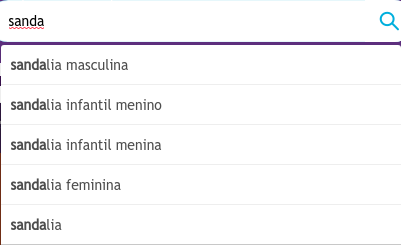
\includegraphics[width=\textwidth]{figures/autocomplete_example1.png}
        \caption{Exemplo de complementação automática de consultas comum.}
        \label{fig:common_autocomplete}
    \end{subfigure}
    \begin{subfigure}[b]{0.49\textwidth}
        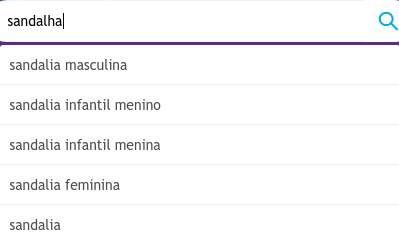
\includegraphics[width=\textwidth]{figures/autocomplete_example2.png}
        \caption{Exemplo de complementação automática de consultas tolerante a erros.}
        \label{fig:error_tolerant_autocomplete}
    \end{subfigure}
    \caption{Complementação automática de consultas em uma plataforma de \textit{e-commerce}. }
    \label{fig:query_autocompletion_example}
\end{figure}


A complementação automática de consultas pode ocorrer de duas formas. A primeira está representada na Figura~\ref{fig:common_autocomplete}, na qual o usuário insere o prefixo de consulta \textit{``sanda''} e o sistema automaticamente sugere cinco possíveis consultas relacionadas cujos prefixos correspondem exatamente ao que foi consultado (destacados em negrito em cada consulta). No entanto, é comum que haja erros de ortografia no conteúdo digitado. Cerca de $10\%$ a $20\%$ das consultas são digitadas erroneamente \citep{broder2009}. Para tratar tais situações é necessário que esses erros sejam considerados na busca pelas sugestões que serão retornadas. Esse problema é denominado complementação automática  tolerante a erros (CATE). Quando o usuário não sabe escrever corretamente uma palavra é provável que ele consulte por um prefixo que contenha erros de digitação. A segunda forma da complementação automática, presente na Figura~\ref{fig:error_tolerant_autocomplete}, representa uma resolução para esse problema. Apesar da digitação errada do prefixo \textit{``sandalha''} o sistema ainda assim foi capaz de exibir sugestões cujos prefixos correspondem aproximadamente ao que foi consultado, pois sua complementação automática de consultas é tolerante a erros. Tal tolerância pode economizar os esforços do usuário de $40\%$ até $60\%$ \citep{ji2009efficient}.

Esse mecanismo pode ser visto como uma versão especializada do problema de casamento de padrão. Nesse problema há uma janela de busca com o mesmo tamanho do padrão $p$ buscado que é movida da esquerda para a direita em um texto $t$. A cada movimento, o padrão $p$ é buscado dentro dessa janela. Esse casamento de padrão pode ser realizado de forma exata, ou aproximada. O problema de casamento exato de padrão é definido como encontrar todas as ocorrências $t_{j',j} = t_{j'}..t_{j}$ de um padrão $p = p_{1},..,p_{m}$ em um texto $t = t_{1},..,t_{n}$, sendo $m \leq n$ \citep{farostringmatching2013}.  

Já o problema de casamento aproximado de padrão é definido como encontrar todas as sub-cadeias de caracteres $t_{j',j} = t_{j'}..t_{j}$ de um texto $t = t_{1},..,t_{n}$ cuja distância de edição para um padrão $P = p_{1},..,p_{m}$ esteja dentro de um limiar $\tau$, ou seja, $ed(t_{j',j}, P) \leq \tau$, sendo $ed(s_{1}, s_{2})$ uma função que calcula a distância de edição entre $s$ e $t$. A distância de edição entre duas cadeias de caracteres $s_{1}$ e $s_{2}$ é definida como \textit{o menor número de operações necessárias para transformar $s_{1}$ em $s_{2}$}. Comumente as operações permitidas nesse contexto são a \textit{inserção}, \textit{deleção} ou \textit{substituição} de um caractere.

Essa versão aproximada do problema de casamento de padrão pode ser aplicada ao problema de CATE. Seja $p$ um prefixo de consulta digitado pelo usuário, $S=\{Q_{1}, Q_{2}, ... , Q_{n}\}$ um conjunto de $n$ cadeias de caracteres que representa todas as possíveis sugestões de consulta, e $\tau$ um limite máximo de distância de edição tolerado. O problema de CATE consiste em encontrar um subconjunto de sugestões $S'$ cujos elementos correspondem à $p$ com no máximo $\tau$ erros. Ou seja, é preciso que cada consulta presente em $S'$ possua pelo menos um prefixo que possa possa ser transformado em $p$ com no máximo $\tau$ operações de edição.

Para exemplificar, seja $\tau = 2$, $p = ``sapatho"$ e S = \textit{\{``sapatilha\ preta'', ``salaminho\ italiano'', ``sapinho\ verde''\}}. De acordo com a definição apresentada acima, o subconjunto de $S$ correspondente às consultas que serão sugeridas será \textit{S' = \{``sapatilha\ preta'', ``sapinho\ verde''\}}. No caso da consulta ``salaminho\ italiano'', seus possíveis prefixos são \textit{\{``s'', ``sa'', ``sal'', ``sala'', ... , ``salaminho italiano''\}}, e nenhum deles pode ser transformado em $p = ``sapatho"$ com no máximo $\tau = 2$ edições, portanto, ela não pode ser retornada como resposta. Por outro lado, a consulta ``sapatilha\ preta'' possui como um de seus prefixos ``sapat'', que pode ser transformado em $p$ com a inserção dos caracteres ``h'' e ``o'' no final (duas operações de inserção). Há também a consulta ``sapinho\ verde'' com o prefixo ``sapinho'', que pode ser transformado em $p$ ao substituir a quarta e quinta letra por ``a'' e ``t'', respectivamente.

A tendência comum entre os melhores métodos propostos recentemente no estado da arte para solucionar esse problema \citep{chaudhuri2009extending,ji2009efficient,li2011efficient, xiao2013efficient,deng2016meta, zhou2016beva} é a de utilizar uma estrutura chamada  \textit{Trie} \citep{fredkintrie1960} para indexar os textos das sugestões de consulta. A \textit{Trie} é uma árvore \textit{M-ária} cujos nós são vetores de tamanho $M$ contendo em suas células caracteres que pertencem a um alfabeto $\Sigma$. O nó raiz $\epsilon$ representa uma cadeia de caracteres vazia. Cada nó em um nível $l$ representa o conjunto de todos os elementos que começam com uma sequência $p$ (que pode ser obtida ao caminhar partindo do nó $\epsilon$ até o nó em questão) de $l$ caracteres. Sendo assim, todos os prefixos em comum dentre os itens indexados compartilham dos mesmos nós. Quando o usuário faz uma consulta por um prefixo, esses métodos utilizam a \textit{Trie} para calcular todos os prefixos similares, e a partir deles sugerir as consultas.

Porém, uma vez que cada nó da árvore pode ter até $|\Sigma|$ filhos, essa estrutura tende a consumir alta quantidade de memória quando a base de consultas indexada é muito grande e não há muitos prefixos em comum entre os itens. Essa situação pode dificultar o uso desses métodos para solucionar o problema de CATE em alguns casos. O método ICAN \citep{ji2009efficient}, por exemplo, ao indexar uma base de aproximadamente $10$ milhões de itens consome $\sim9GB$ de memória. Além disso, o complemento automático de consultas em sistemas de busca deve ocorrer muito rapidamente, de forma quase imperceptível para o usuário. Para isso, cada complementação deve ocorrer em menos de $100ms$ \citep{ji2009efficient}.

Uma possível abordagem para diminuir o uso de memória utilizada para processar as consultas é a estratégia de busca em dois níveis. No primeiro nível é possível realizar a busca em um índice \textit{Trie} que indexa somente uma parte inicial dos textos da base de sugestões de consulta. As folhas encontradas por essa busca podem estar associadas com um conjunto de itens, em vez de um único texto (restante da sugestão de consulta). Então, no segundo nível, cada elemento desse conjunto é analisado (um por um, de forma sequencial) para determinar quais sugestões desse conjunto de fato vão ser sugeridas. 

Costa Xavier \citep{xavier2019} realizou um trabalho preliminar que confirmou a hipótese de que é possível utilizar uma abordagem de busca em dois níveis para o problema de complementação automática de consultas tolerante a erros. Em sequência, Gama Ferreira \citep{berg2020} aprimorou significativamente a busca em dois níveis ao utilizar utilizar o mesmo algoritmo (BEVA) de busca nos dois níveis da \textit{Trie} e ao apresentar uma nova estratégia de inserção de chaves em seu índice que acelera o processamento das consultas por utilizar o sistema de cache das máquinas de maneira mais eficiente. % ideia do "level at a time" -> muito boa :)!

A abordagem em dois níveis pode proporcionar uma ótima redução consumo de memória como dito anteriormente. No entanto, um dos maiores problemas com essa abordagem é o aumento do tempo de processamento necessário para sugerir consultas para um prefixo, pois a classe de complexidade computacional da busca sequencial realizada no segundo nível normalmente está acima da classe de complexidade dos algoritmos de busca que podem ser utilizados nas árvores \textit{Trie} do primeiro nível.

Neste trabalho estudamos alternativas para otimizar a busca em uma abordagem de dois níveis com o objetivo de computar as complementações de consulta tolerando erros, mantendo um bom desempenho aliado à redução da memória utilizada. Investigamos os impactos de uma heurística que visa aproveitar informações de erros de distância de edição provenientes do processamento da consulta no primeiro nível para acelerar o processamento no segundo nível, estudando seus efeitos no tempo de processamento e na acurácia de resultados (medição de quantas sugestões o método deixou de encontrar e quantas sugestões encontradas na verdade não deveriam ser consideradas). 

Para implementar as ideias propostas utilizamos no primeiro nível o algoritmo ICPAN \citep{li2011efficient}, o qual é uma otimização do algoritmo ICAN \citep{ji2009efficient}, para realizar a busca no índice \textit{Trie}. Ambos utilizam uma estratégia incremental que consiste em processar um prefixo de consulta $p=c_{1}c_{2}...c_{x}$ caractere a caractere, e ``ativar'' nós da árvore \textit{Trie} a cada etapa do processamento. Para o i-ésimo caractere processado, cada nó ativo $n$ representa um prefixo cuja distância de edição $\xi_{n}^{p'}$ entre $p'=p[c_{1}..c_{i}]$ é menor ou igual ao limite de tolerância $\tau$ estabelecido. O ICPAN é mais eficiente que o ICAN pois utiliza um conceito de ``nós ativos pivotais'' para reduzir o conjunto de nós ativados durante toda a computação. Essa redução implica que menos itens precisarão ser verificados no segundo nível, e portanto é vantajosa para a abordagem em dois níveis.

Quanto ao segundo nível, criamos a hipótese de que é possível em alguns casos realizar uma busca binária em vez de uma busca sequencial. Então, estudamos o quão efetiva seria uma abordagem que combina a estratégia de realizar tanto buscas sequenciais quanto binárias no segundo nível. Descobrimos no decorrer da pesquisa que apesar dessa estratégia atingir tempos de processamento até 2 vezes mais rápidos do que a abordagem padrão de dois níveis, ela faz o método recuperar itens que não devia, e também o faz deixar de recuperar itens relevantes. No entanto, ao tolerar $\tau=3$ erros de digitação na busca, os métodos que utilizam busca binária podem apresentar bons níveis de acurácia.

\section{Problema de Pesquisa}
\label{sec:research-problem}
A principal hipótese estudada nesta dissertação é a de que é possível implementar um sistema de complementação automática em dois níveis combinando busca sequencial e busca binária no segundo nível, de forma que a eficiência do processamento aumente e que a acurácia dos resultados não seja prejudicada. As propostas apresentadas por \cite{xavier2019} e \cite{berg2020} indicam que a busca em dois níveis é uma abordagem promissora para sistemas de complementação automática. Ao iniciar esta pesquisa, tivemos a ideia de combinar busca binária com sequencial no segundo nível. Apesar de parecer uma ideia simples a princípio, sua implementação trouxe consigo desafios que são apresentados ao longo do trabalho. Nossa pesquisa teve como objetivo responder às seguintes questões de pesquisa: i) É possível adaptar sistemas de busca em dois níveis para tirarem proveito da busca binária no segundo nível? ii) Quais são as adaptações necessárias e limitações de uso da ideia? iii) Há vantagens práticas na combinação de busca binária e busca sequencial no segundo nível?


O restante desta dissertação está organizado da seguinte forma: No Capítulo~\ref{sec:related_work} nós mostramos os trabalhos relacionados e os algoritmos existentes na literatura que abordam o problema de complementação automática de consultas tolerante a erros. No Capítulo~\ref{sec:ref_teorico} introduzimos uma definição formal do problema e apresentamos alguns conceitos necessários para uma compreensão mais completa do trabalho. No Capítulo~\ref{sec:metodo} detalhamos a implementação dos métodos em dois níveis propostos. No Capítulo~\ref{sec:results} apresentamos e analisamos os resultados dos experimentos realizados, e por fim, no Capítulo~\ref{sec:conclusion}, expomos nossas conclusões do trabalho e também possíveis direções para trabalhos futuros.

\newpage
\thispagestyle{empty}
\mbox{}
\newpage

% ---------------------
% Trabalhos relacionados
% ---------------------
\chapter{Trabalhos relacionados}\label{sec:referencias}
\label{sec:related_work}

O problema de CATE foi primeiramente estudado por \cite{chaudhuri2009extending} e \cite{ji2009efficient}. Ambos propuseram soluções baseadas em computar, de forma incremental, um conjunto de nós ativos de uma \textit{Trie}, a qual funciona como índice para a base de consultas que poderão ser sugeridas. A ideia geral comum entre os dois algoritmos é a de que os algoritmos calculam um conjunto de ``nós ativos'' que correspondem a todos os prefixos encontrados na \textit{Trie} similares a cada letra nova de um prefixo de consulta $p$ digitado pelo usuário, dentro de um limite de distância de edição $\tau$. A partir desses prefixos calculados, é possível recuperar na própria árvore o restante do texto das consultas que serão sugeridas.

Chaudhuri et al. \cite{chaudhuri2009extending} apresentam um método de complementação automática de consultas que leva em consideração erros de digitação no prefixo. Antes disso, para cenários em que havia uma tabela de frases para pesquisar, a forma mais comum de preenchimento automático era a comparação exata de caracteres. Dois algoritmos de complementação automática tolerantes à falha de digitação foram propostos \citep{chaudhuri2009extending}. O primeiro é baseado nos algoritmos de distância de edição em q-gramas\citep{arasu2006efficient, chaudhuri2006primitive, xiao2008ed}. O segundo é um algoritmo baseado em \textit{Trie}, que mantém um conjunto de \textit{nós ativos} de forma incremental para processar as complementações. O método utiliza distância de edição clássica como medida de similaridade entre cadeias de caracteres. Esse algoritmo é muito similar ao proposto por \cite{ji2009efficient}, porém, realiza uma etapa a mais, que consiste em pré-computar o conjunto de nós ativos para todas as possíveis consultas com até certo tamanho. Uma vez que o número de nós ativos pode ser muito grande ao realizar complementação de consultas tolerante a erros, essa estratégia ajuda a reduzir o tempo de processamento das consultas.

Para abordar o problema de CATE Ji et. al \citep{ji2009efficient} propõem um algoritmo chamado \textit{ICAN} que computa nós ativos de forma incremental, ou seja, processa o prefixo consultado caractere a caractere, como mencionado anteriormente. Nosso método proposto na seção~\ref{sec:metodo} utiliza uma otimização desse algortimo, o ICPAN \citep{li2011efficient}. Portanto, ambos serão descritos com mais detalhes a seguir, e também serão mais aprofundados na seção~\ref{sec:ref_teorico}. 

Seja $p$ um prefixo consultado e $\tau$ um limite de distância de edição. Um nó $n$ da \textit{Trie} é chamado \textit{nó ativo de p em relação à $\tau$} quando a distância de edição entre a cadeia de caracteres de $n$ e a de $p$ estiver dentro do limite $\tau$, ou em outras palavras, $ed(n, p) \leq \tau$. Os nós-folha da subárvore com raiz em $n$ são denominados ``palavras similares à $p$'' \citep{ji2009efficient}. 

Considerando uma consulta de prefixo $p$ com apenas uma palavra-chave, para processar os nós ativos de forma eficiente é necessário computar e armazenar um conjunto de tuplas $\Phi_{p} = \{ \langle n, \xi_{n} \rangle \}$ tal que (1) cada $n$ é um nó ativo em relação à $p$ com $\xi_{n} = ed(n, p) \leq \tau)$ e (2) quaisquer nós ativos de $p$ estão presentes em $\Phi_{p}$, que é o \textit{conjunto de nós ativos de p} \citep{ji2009efficient}. Quando o usuário digita mais um caractere $p + 1$ após ter digitado $p$, o conjunto $\Phi_{p}$ de nós ativos de $p$ pode ser usado para computar o conjunto $\Phi_{p + 1}$ de nós ativos da nova consulta.

Uma desvantagem do algoritmo ICAN é que pode ser bastante custoso manter o conjunto de nós ativos para grandes quantidades de dados. Para atenuar esse problema, Li et al. \citep{li2011efficient} desenvolveram um método otimizado denominado \textit{ICPAN}, que realiza a poda de nós ativos desnecessários durante o processamento de consultas enquanto continua conseguindo computar todos os itens similares ao prefixo consultado. Isso permite a redução do espaço necessário para armazenar os nós ativos computados e também melhora o desempenho da busca, uma vez que não é necessário verificar todos os nós ativos para a computação incremental.

O ICPAN define um subconjunto dos nós ativos que pode ser usado para computar todas as palavras similares à consulta de forma eficiente e incremental. Para isso, Li et al. \citep{li2011efficient} estabelecem a seguinte observação: dado um nó ativo $n$ de $p$, se para qualquer transformação de $n$ para $p$ com $ed(n,p)$ operações de edição, não houver uma operação de correspondência (caracteres iguais) no último caractere de $n$, e for possível deletar o último caractere de $n$, o nó $n$ não é mantido, e sim o seu nó pai. Assim, surge o conceito de \textit{nó pivô ativo}.

Considerando um prefixo de consulta $p$, um nó da \textit{Trie} $n$ é um nó pivô ativo de $p$ em relação à $\tau$ se, e somente se (1) $n$ é um nó ativo de $p$ e (2) se existe uma transformação de $p$ para $n$ com $ed(n,p)$ operações, e a operação no último caractere de $n$ é uma correspondência. Em outras palavras, a operação nesse caractere de $n$ não é nem uma deleção $ed(n,p) \neq ed(n',p) + 1$ e nem uma substituição $ed(n,p) \neq ed(n', p') + 1$, onde $n'$ e $p'$ são respectivamente os prefixos de $n$ e $p$ que não contêm o último caractere.

Dada uma consulta de prefixo $p_{x}$, de forma análoga ao ICAN, é preciso computar e armazenar um conjunto de tuplas $\Psi_{p_{x}} = \{ \langle n, \xi_{n}^{p_{x}}, p_{i}, \xi_{n}^{p_{i}} \rangle \}$ \citep{li2011efficient}. Em cada tupla, $n$ é um nó pivô ativo de $p_{x}$. O elemento $p_{i}$ é um prefixo de $p_{x}$ tal que os últimos caracteres de $n$ e $p_{i}$ são iguais. Se não existir tal prefixo, então $p_{i} = \epsilon$ (cadeia de caracteres vazia). Se existirem múltiplos prefixos com essa condição, somente aquele com o menor comprimento é selecionado. $\xi_{n}^{p_{i}} \leq \tau$ é uma distância de transformação entre o nó $n$ para $p_{i}$ com uma operação de correspondência entre seus últimos caracteres. $\xi_{n}^{p_{x}} \leq \tau$ é a distância de transformação entre o nó $n$ para $p_{x}$ obtida ao primeiro transformar o nó $n$ para $p_{i}$ e então inserir os caracteres após $p_{i}$. O ICPAN é um algoritmo que computa $\Psi{p_{x}}$ e garante que cada nó pivô ativo de $p_{x}$ aparece como o $n$ em uma tupla de $\Psi{p_{x}}$.

Em contrapartida, Xiao et al. \citep{xiao2013efficient} argumentam que a eficiência dos métodos supramencionados criticamente depende da quantidade de nós ativos, e que tal número é tipicamente muito grande e também linear no tamanho da base de sugestões indexada, ou até mesmo exponencial no tamanho do alfabeto no pior caso. Então, os autores resolvem seguir em outra direção, investigando se é possível melhorar drasticamente o desempenho do processamento da consulta ao processar previamente a base e construir um índice de grandes proporções. Para isso, propuseram uma solução denominada IncNGTrie que consiste em indexar as ``variações marcadas de deleção'' (VMD) das sugestões em uma Trie e então manter um pequeno conjunto de nós ativos durante o processamento. 

O conteúdo indexado não é o texto original das sugestões de consulta e sim suas variantes marcadas de $\tau$-deleções, as quais são geradas ao deletar no máximo $\tau$ caracteres dos textos. Então, quando o usuário digita uma consulta o método computa as variantes da mesma e as pesquisa na árvore Trie. Essa técnica pode ser realizada de forma incremental e eficiente, mantendo um pequeno conjunto de nós ativos (reduzindo o tamanho em até 3 ordens de grandeza comparado aos métodos ICAN e ICPAN, por exemplo). 
Apesar dessa abordagem ter reduzido o tempo necessário para processar as consultas em comparação às outras soluções presentes na literatura, o tamanho dos índices também se demonstrou muito maior que dos outros métodos, representando uma severa restrição à utilização do IncNGTrie quanto à memória. Qin et al. \citep{qin2020efficient} apresentam o IncNGTrie+, uma melhoria do IncNGTrie que reduziu tanto o tempo de processamento quanto o tamanho do índice construindo, diminuindo a quantidade de memória requerida, apesar de ainda precisarem de mais memória do que os métodos BEVA e META, por exemplo.

Zhou et al. \citep{zhou2016beva} propõem uma estrutura geral que engloba métodos da complementação automática existentes, o ``BEVA'', caracterizando diferentes classes de algoritmos e a quantidade mínima de informações que eles precisam manter para diversas restrições. É proposta também uma nova estratégia de armazenamento de ``nós ativos de fronteira'' (menor conjunto de nós ativos possível, sem redundâncias), eliminando inteiramente os relacionamentos entre nós pais e filhos. Essa abordagem realiza computação de distância de edição através de uma nova estrutura de dados chamada ``\textit{edit vector automaton}'' (EVA), conseguindo calcular novos nós ativos e seus estados associados de forma eficiente através de pesquisas de tabela. O modelo é capaz de suportar limiares de grande distância através de um autômato. Os estudos do trabalho indicam que o método supera as abordagens até então existentes, tanto em tempo quanto na eficiência do espaço.

Deng et al. \citep{deng2016meta} desenvolveram um método denominado ``META'', uma estrutura baseada em correspondências que calcula as respostas com base em caracteres correspondentes entre os dados das consultas e os dados indexados. A estrutura desenvolvida é capaz de reduzir cálculos redundantes, organizando-os através de índices de árvore compacta. Para processar as respostas às consultas foi proposto um método incremental que responde eficientemente consultas \textit{top-k}. 

Todos os trabalhos supracitados utilizam \textit{Trie} como seu principal índice para realizar a computação de prefixos similares ao prefixo de consulta digitado pelo usuário. Isso fornece uma forte base para considerar que essa estrutura de dados realmente é vantajosa para o problema de CATE em se tratando do tempo de processamento. No entanto, as árvores \textit{Trie} tendem a consumir uma alta quantidade de memória quando a base de consultas indexada é muito grande e não há muitos prefixos em comum entre os itens. Uma das formas de contornar esse problema é utilizar uma estratégia de indexação e busca em dois níveis.

Manber et al. \citep{manber1994glimpse} apresentam o ``GLIMPSE'' (\textit{GLobal IMPlicit Search}) ou ``Busca Implícita Global'', uma ferramenta que possibilita a realização de consultas para sistemas de arquivos com baixa indexação, onde apenas 2\% e 4\% do tamanho do texto é indexado. O GLIMPSE apresentou uma abordagem até então nova para a indexação e realização de consultas de arquivos, denominada de ``busca em dois níveis''.

A ideia da busca em dois níveis aplicada no GLIMPSE consiste em combinar índices invertidos completos com busca sequencial sem indexação. Essa abordagem se baseia na observação de que a busca sequencial é rápida o suficiente para textos de vários \textit{megabytes} de tamanho, e que por isso não é necessário indexar todas as palavras do documento com suas localizações exatas. Na busca em dois níveis, o índice não fornece os locais exatos das palavras, mas apenas uma indicação da região onde a resposta possa ser encontrada, funcionando como uma espécia de ``filtro''. Nessa abordagem no entanto, apesar de economizar bastante espaço de indexação, a velocidade de busca se mostrou inferior aos modelos que utilizam apenas indexadores baseados em lista invertida.

Navarro et al. ~\citep{navarro2000adding} estudaram uma possível combinação entre índice invertido completo e pesquisa sequencial sem indexação. A pesquisa completa em coleções de texto é feita com o uso de um índice que aponta para blocos em vez de apontar para cada posição no texto. Primeiramente, a pesquisa é realizada no índice para detectar blocos que podem corresponder à consulta e, em seguida, no segundo nível é feita uma pesquisa sequencial para encontrar a lista real de
ocorrências no texto.

Quanto ao índice utilizado no primeiro nível, é possível utilizar índices baseados em árvores \textit{Trie}. Heinz et al. \citep{heinz2002burst} propõem a estrutura \textit{Burst Trie}, a qual pode ser considerada como um outro exemplo de índice de dois níveis, porém é aplicada em outro contexto. As \textit{Burst \textit{Trie}s} são coleções de pequenas estruturas de dados denominadas ``recipientes''. Esses ``recipientes'' são análogos ao segundo nível nos moldes explicados anteriormente, e são acessados através de uma \textit{Trie} comum, a qual pode ser considerada como um primeiro nível.

Um problema comum a todos os métodos de complementação automática de consultas tolerante a erros supracitados é o alto consumo de memória, uma vez que todos utilizam a estrutura \textit{Trie} para indexar todo o texto de cada consulta da base de dados. Tendo como influência a combinação de índice invertido e pesquisa sequencial sem indexação (``busca em dois níveis''), uma forma de reduzir a quantidade de memória necessária seria indexar somente alguns caracteres iniciais de cada consulta na árvore \textit{Trie}, e utilizar de pesquisa sequencial caso o processamento precise ir além das folhas da árvore. 

Costa Xavier \citep{xavier2019} realizou um trabalho preliminar que confirmou ser possível utilizar uma abordagem de busca em dois níveis para o problema de CATE. Nesse método, define-se uma quantidade fixa $L$ de caracteres (profundidade máxima da \textit{Trie}), e então somente os $L$ primeiros caracteres de cada consulta são indexados na árvore. Dado um prefixo de consulta $P$ tal que $|P| > L$, a computação de sugestões é dividida em duas etapas, ou níveis. O primeiro nível utiliza o algoritmo ICAN \citep{ji2009efficient} para processar os $L$ primeiros caracteres de $P$. Após o término, resta um conjunto de nós ativos da \textit{Trie} referentes à sub-cadeia  $P[1..L]$. Então, no segundo nível, é realizada uma busca sequencial em cada consulta referenciada por cada nó ativo. 

Após esse primeiro trabalho, Gama Ferreira \citep{berg2020} aprimorou significativamente a busca em dois níveis ao utilizar utilizar o mesmo algoritmo (BEVA) de busca nos dois níveis da \textit{Trie}. Além disso, o trabalho propõe uma estratégia de inserção de chaves em seu índice \textit{Trie} que acelera o processamento das consultas por utilizar o sistema de cache das máquinas de maneira mais eficiente. Essa mudança na forma de inserir chaves tem potencial para causar melhorias também em outros algoritmos baseados em \textit{Trie} presentes na literatura. A busca sequencial no segundo nível deste método é mais eficiente que a de \cite{xavier2019}, porque os estados de computação de distância de edição já existentes no primeiro nível podem ser usados para poupar redundâncias computacionais no segundo nível. Tal método atingiu uma ótima economia de memória em comparação ao algoritmo original BEVA, com o aditivo de conseguir manter um desempenho semelhante. 

Os trabalhos de \cite{xavier2019} e \cite{berg2020} demonstraram que é possível combinar a estratégia de busca em índices \textit{Trie} com busca sequencial para resolver o problema de CATE. Tal combinação reduz significativamente o uso de memória, enquanto mantém o tempo de processamento dentro do limite ideal de $100ms$ para uma boa parte dos casos experimentados. Nesta dissertação, exploramos a possibilidade de realizar otimizações em alguns casos específicos de processamento de consultas no segundo nível ao combinar busca sequencial com busca binária, visando obter ganhos de desempenho.

\newpage
\thispagestyle{empty}
\mbox{}
\newpage

% ---------------------
% Referencial Teórico
% ---------------------
\section{Referencial Teórico}\label{sec:ref_teorico}

O problema de casamento de padrão consiste em buscar as ocorrências de uma dada cadeia de caracteres $p$ em um texto $t$. Nele há uma janela, na qual o padrão é buscado, que possui o mesmo tamanho do padrão e é movida da esquerda para a direita pelo texto.

Há dois tipos de problemas de casamento de padrão:
\begin{itemize}
    \item Casamento exato de padrão
    \item Casamento aproximado de padrão
\end{itemize}

O problema de casamento exato de padrão é definido como encontrar todas as ocorrências $t_{j',j} = t_{j'}..t_{j}$ de um padrão $p = p_{1},..,p_{m}$ em um texto $t = t_{1},..,t_{n}$, sendo $m \leq n$.

Já o problema de casamento aproximado de padrão é definido como encontrar todas as subcadeias de caracteres $t_{j',j} = t_{j'}..t_{j}$ de um texto $t = t_{1},..,t_{n}$ cuja distância de edição para um padrão $P = p_{1},..,p_{m}$ esteja dentro de um limiar $\tau$, ou seja, $ed(t_{j',j}, P) \leq \tau$, sendo $ed(s_{1}, s_{2})$ uma função que calcula a distância de edição entre $s$ e $t$. Nesse caso, o tamanho de cada ocorrência pode variar de $m - \tau$ até $m + \tau$. A distância de edição entre duas cadeias de caracteres $s_{1}$ e $s_{2}$ é definida como \textit{o menor número de operações para transformar $s_{1}$ em $s_{2}$}. As operações mais permitidas comumente nesse contexto seguem a chamada \textit{distância de edição de Levenshtein} \citep{levenshtein1966binary}, que são:

\begin{enumerate}
    \item \textbf{Inserção} de um único caractere. Se $s = ac$ então inserir o símbolo $b$ na posição do meio, por exemplo, produz $s = abc$. Também pode ser representada por $\epsilon \to b$.
    \item \textbf{Deleção} de um único caractere torna $s = abc$ em $s = bc$, por exemplo. Também pode ser representada por $a \to \epsilon$.
    \item \textbf{Substituição} de um caractere $b$ por um símbolo $q \neq b$ modifica  $s = abc$ para $s = aqc$. Também pode ser representada por $b \to q$.
\end{enumerate}

Esse problema é encontrado em  várias aplicações práticas,  por exemplo em buscas por sequências de DNA, ou para prover sugestões de correções de erros de digitação cometidos pelos usuários ao realizarem consultas em sistemas de busca.

\newpage
\subsection{Problema da Complementação Automática de Consultas Tolerante a Erros}

O problema de complementação automática de consultas tolerante a erros pode ser visto como uma versão especializada do problema de casamento de padrão. Seja \textit{p} uma cadeia de caracteres que representa uma consulta de prefixo já digitada pelo usuário, um conjunto de cadeias de caracteres \textit{S} que representa a base de consultas e $\tau$ um limite máximo de distância de edição tolerado. O problema consiste em encontrar todos os elementos de \textit{S} que correspondem à \textit{p} com no máximo $\tau$ erros.

Um elemento $s$ qualquer do conjunto $S$ possui vários prefixos. Se $s = ``sapato"$, seus possíveis prefixos são \textit{\{``s'', ``sa'', ``sap'', ``sapa'', ``sapat'', ``sapato''\}}. Se qualquer um deles puder ser transformado em $p$ com um número de operações menor ou igual à $\tau$, então $s$ corresponde à $p$ com no máximo $\tau$ erros, e fará parte da resposta do problema. A solução para o problema deve atender a uma restrição de computar os resultados em um tempo menor que a velocidade média de digitação de um usuário comum, a qual é aproximadamente $100ms$ \citep{ji2009efficient}.

\subsection{Opções de Solução para o Problema de CATE}

As soluções para o problema de casamento de padrão podem ser divididas em dois grupos. O primeiro engloba abordagens baseadas em busca sequencial por toda a base de consultas. O segundo grupo consiste em abordagens que criam índices a partir da base de consultas em um momento anterior ao processamento de requisições. 

\subsubsection{Busca Sequencial}
\label{sec:sequential_search}

Os algoritmos de busca sequencial que não utilizam índices consistem em percorrer todos os itens da base de consultas, e comparar o prefixo de consulta com cada item, para determinar quais consultas devem fazer parte da resposta. No contexto de CATE, essa comparação consiste em verificar se o prefixo consultado pode ser transformado em algum dos possíveis prefixos da consulta com no máximo $\tau$ operações. Descreveremos a seguir uma solução de busca sequencial baseada em um algoritmo de programação dinâmica proposto por \cite{levenshtein1966binary}. 

Um método conhecido para calcular a distância de edição entre duas cadeias de caracteres $A$ e $B$, com tamanhos $n$ e $m$ respectivamente, é o algoritmo de programação dinâmica que preenche uma matriz $M$ de tamanho $(n + 1) \cdot (m + 1)$. Cada célula $M[i,j]$ armazena a distância de edição entre os prefixos de tamanho $i$ e $j$ das cadeias $A$ e $B$, respectivamente. Esses valores podem ser computados ``linha à linha'' ou ``coluna à coluna'' com base na seguinte equação de recorrência:

% \qquad\displaystyle 

\[ 
M[i,j] =
        \begin{cases}
        max(i, j), \text{se}\ min(i, j) = 0 \\
         \min
         \begin{cases}
         M[i - 1, j]  + 1 \\ 
         M[i, j - 1]  + 1 \\ 
         M[i - 1, j - 1] + \delta(A[i], B[j]) \end{cases}
         \end{cases}, \text{senão}
\]

, na qual $\delta(x,y) = 0$ se $x = y$ (sendo $x$ e $y$ caracteres) e $\delta(x,y) = 1$ caso contrário. As condições para os limites da matriz são $M[0, j] = j$ e $M[i, 0] = i$. 

\begin{table}[h]
\centering
\begin{tabular}{lllllll}
 &  & {\color[HTML]{C0C0C0} 0} & {\color[HTML]{C0C0C0} 1} & {\color[HTML]{C0C0C0} 2} & {\color[HTML]{C0C0C0} 3} & {\color[HTML]{C0C0C0} 4} \\
 &  & $\epsilon$ & \textbf{c} & \textbf{a} & \textbf{p} & \textbf{a} \\ \cline{3-7} 
{\color[HTML]{C0C0C0} 0} & \multicolumn{1}{l|}{$\epsilon$} & \multicolumn{1}{l|}{0} & \multicolumn{1}{l|}{1} & \multicolumn{1}{l|}{2} & \multicolumn{1}{l|}{3} & \multicolumn{1}{l|}{4} \\ \cline{3-7} 
{\color[HTML]{C0C0C0} 1} & \multicolumn{1}{l|}{\textbf{s}} & \multicolumn{1}{l|}{1} & \multicolumn{1}{l|}{1} & \multicolumn{1}{l|}{2} & \multicolumn{1}{l|}{3} & \multicolumn{1}{l|}{4} \\ \cline{3-7} 
{\color[HTML]{C0C0C0} 2} & \multicolumn{1}{l|}{\textbf{a}} & \multicolumn{1}{l|}{2} & \multicolumn{1}{l|}{2} & \multicolumn{1}{l|}{1} & \multicolumn{1}{l|}{2} & \multicolumn{1}{l|}{3} \\ \cline{3-7} 
{\color[HTML]{C0C0C0} 3} & \multicolumn{1}{l|}{\textbf{p}} & \multicolumn{1}{l|}{3} & \multicolumn{1}{l|}{3} & \multicolumn{1}{l|}{2} & \multicolumn{1}{l|}{1} & \multicolumn{1}{l|}{2} \\ \cline{3-7} 
{\color[HTML]{C0C0C0} 4} & \multicolumn{1}{l|}{\textbf{o}} & \multicolumn{1}{l|}{4} & \multicolumn{1}{l|}{4} & \multicolumn{1}{l|}{3} & \multicolumn{1}{l|}{2} & \multicolumn{1}{l|}{2} \\ \cline{3-7} 
\end{tabular}
\caption{Cálculo de distância de edição entre o prefixo de consulta ``capa'', e a sugestão de consulta ``sapo'' com a matriz de programação dinâmica.}
\label{tab:levenhstein_matrix_sequential_search}
\end{table}

A Tabela~\ref{tab:levenhstein_matrix_sequential_search} demonstra a matriz $M$ resultante para o cálculo de distância entre o prefixo de consulta $p = ``capa"$, e a sugestão $s = ``sapo"$. Nela, a primeira coluna e a primeira linha são referentes a uma cadeia de caracteres vazia, representada por $\epsilon$. Para obter a distância de edição basta considerar o valor de $M[|p|, |s|] = 2$. A complexidade de tempo para calcular a matriz completa é $O(n \cdot m)$. 

Ainda considerando o exemplo presente na Tabela~\ref{tab:levenhstein_matrix_sequential_search}, precisamos atentar para a última coluna $M[i, |p|]$ da matriz. O elemento $M[0, |p|]$ é referente à distância de edição entre ``capa'' e uma palavra vazia ``''. Já os elementos $M[1, |p|]$ e $M[2, |p|]$ são respectivamente referentes à distância entre ``capa`` e ``s'', e à distância entre ``capa'' e ``sa'', e assim sucessivamente. Para o problema de CATE, basta que qualquer valor de $M[i, |p|] \leq \tau$ para que uma consulta $s$ seja considerada como resposta para o problema. Devido a isso, uma vez que essa matriz é calculada de cima para baixo e da esquerda para direita, é possível interromper o processamento caso um valor calculado para a última coluna seja menor ou igual a $\tau$, e já considerar o item como resposta. Se $\tau = 3$ por exemplo, quando o elemento $M[2, 4] = 3$ é calculado na Tabela~\ref{tab:levenhstein_matrix_sequential_search}, a sugestão ``sapo'' já pode ser considerada como resposta para o prefixo de consulta ``capa'', pois $M[2, 4] \leq \tau$, e então não é mais necessário calcular as linhas 3 e 4 da matriz.

Seja $\mc{S}$ um conjunto de sugestões de consulta, $p$ um prefixo de consulta digitado pelo usuário, $\tau$ um limiar de erros de digitação tolerados, e $Respostas$ um conjunto de sugestões inicialmente vazio. Para cada sugestão $s$ de $S$ aplica-se o procedimento definido acima. Se $s$ contiver um prefixo similar à $p$ com no máximo $\tau$ operações de distância de edição, então é considerada uma sugestão de consulta válida, e adicionada ao conjunto de resposta $Respostas$. Ao final desse processamento, o conjunto $Respostas$ representará um subconjunto de $S$ que contém todos os prefixos similares à $p$ considerando o limiar $\tau$, e portanto, também será considerado a solução do problema de CATE.

Existem algoritmos de busca sequencial mais eficientes em comparação ao que foi apresentado acima, mas o mesmo é importante pois fornece uma base de entendimento para os outros algoritmos mais complexos que estudaremos aqui. 
% No entanto, mesmo as soluções mais eficientes com essa abordagem podem facilmente atingir um alto consumo de memória quando a base é muito grande. Portanto, essas soluções não são aceitáveis em alguns dos cenários de complementação de consultas.

\subsubsection{Busca com Utilização de Índices}

Os métodos baseados em índices utilizam estruturas de dados especiais para diminuir o tempo de processamento das consultas. Há diversas alternativas de estruturas de índices especializadas para o problema de CATE, como por exemplo índices invertidos \citep{baezayates99}, árvores de sufixo, ou árvores \textit{Trie}. Dentre essas estruturas, a mais adotada dentre os algoritmos mais recentes da literatura é a árvore \textit{Trie} \citep{chaudhuri2009extending,ji2009efficient,li2011efficient, xiao2013efficient,deng2016meta, zhou2016beva}.

Mesmo que a solução de busca sequencial não seja viável, Costa Xavier e Gama Ferreira \citep{xavier2019, berg2020} estudaram a possibilidade de combiná-la com métodos baseados em índices, visando obter soluções que economizem memória enquanto mantêm uma boa velocidade de processamento das consultas. Essa abordagem é chamada ``busca em dois níveis'', e utiliza índices para reduzir o espaço de busca e então realiza uma busca sequencial nesse espaço reduzido.

\subsection{Trie}
\label{sec:trie}

A estrutura de dados \textit{Trie} ou ``árvore digital'' é uma árvore que armazena um conjunto de palavras e são capazes de recuperar qualquer termo indexado em um tempo proporcional ao seu comprimento, independentemente do tamanho e quantidade total das palavras armazenadas. Os caracteres das palavras armazenadas nessa estrutura pertencem a um alfabeto predefinido $\Sigma$, e cada nó da árvore contém um caractere armazenado como chave. A estrutura começa com o nó raiz que representa uma palavra vazia $\epsilon$ (palavra com $0$ caracteres). Cada nó possui um conjunto de nós filhos com tamanho menor ou igual a $|\Sigma|$, sendo $|\Sigma|$ o tamanho do alfabeto. Para cada nó da árvore é possível caminhar do nó raiz até o mesmo e computar um prefixo, concatenando os caracteres dos nós presentes nesse caminho. Objetivando a simplicidade, iremos nos referir aos nós pelo seu prefixo correspondente de forma intercambiável.

A inserção de uma nova palavra $K$ começa com uma operação de busca para encontrar o caminho na árvore com o maior número de caracteres em comum com $K$. Essa busca começa definindo o nó raiz nó ``atual'', denotado por $N_{atual}$, e a posição atual $pos$ na palavra inserida como $1$, que representa o primeiro caractere da cadeia. Então, repete-se o procedimento de procurar por algum nó filho de $N_{atual}$ cujo caractere chave é igual a $K[pos]$. Caso esse nó seja encontrado, $N_{atual}$ passará a apontar para ele, e a variável $pos$ é incrementada em $1$. Caso não seja encontrado, cria-se um novo nó filho em $N_{atual}$ com o valor de $K[pos]$ como sua chave, e $N_{atual}$ passa a apontar para esse novo nó, e $pos$ é incrementada em $1$. Esse processo é repetido até que o último caractere de $K$ seja alcançado.

A busca por uma palavra $K$ a na \textit{Trie} consiste em um procedimento parecido com a inserção. No entanto, a busca resulta em falha no momento em que não se encontra um nó filho de $N_{atual}$ com chave igual a $K[pos]$. Quando o algoritmo segue com sucesso até um nó folha da \textit{Trie}, se todos os caracteres de $K$ foram encontrados, então a busca indica que a palavra foi encontrada. Considerando uma busca linear nos conjuntos de nós filhos de cada nó da \textit{Trie}, o custo de busca e inserção de nova palavra é $O(|\Sigma| \cdot m)$, onde $m$ é o tamanho da palavra. Uma característica importante é que esse custo não depende da quantidade de palavras já inseridas na \textit{Trie}, o que torna essa estrutura uma boa opção para a indexação de cadeias de caractere. Além disso, também possibilita busca eficiente por padrões em uma grande base de texto, como ocorre no problema de CATE.

\begin{figure}[ht]
    \centering
    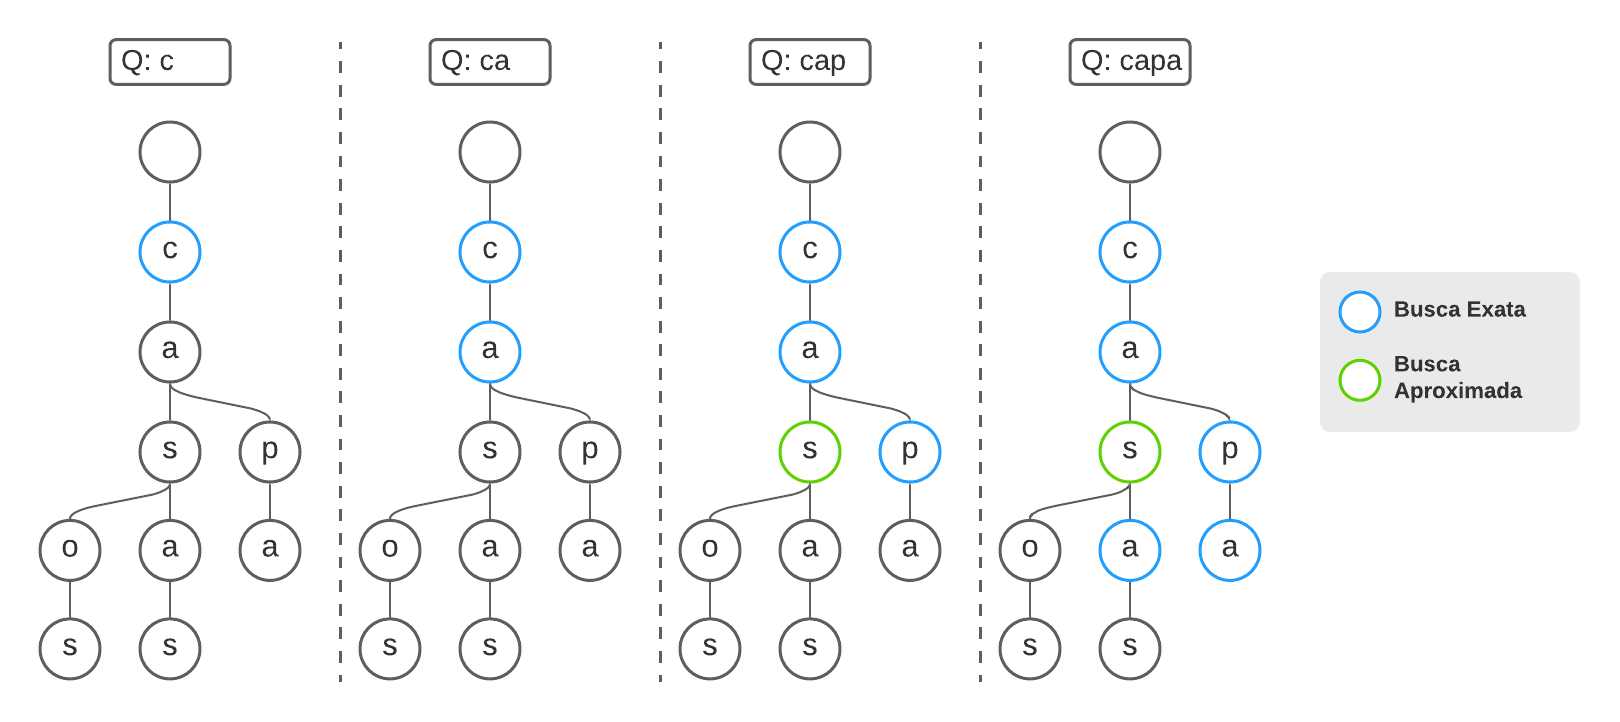
\includegraphics[width=1\textwidth]{figures/trie_exact_and_approximate_search.png}
    \caption{Árvore \textit{Trie} com exemplo de busca exata e aproximada pelo prefixo de consulta ``capa''. Os nós com o contorno azul representam o caminho realizado pela busca exata, e os nós com contorno verde o caminho realizado pela busca aproximada. O caminho da busca aproximada pode conter nós do caminho da busca exata. Esse exemplo considera $\tau = 1$. }
    \label{fig:exact_and_approximate_search_trie}
\end{figure}

Além da busca exata por palavras na \textit{Trie}, também é possível realizar busca aproximada, ou seja, tolerante a erros de digitação. A Figura~\ref{fig:exact_and_approximate_search_trie} mostra um exemplo de busca exata e busca aproximada pelo prefixo de consulta ``capa'' em uma \textit{Trie}. A busca exata consiste em visitar apenas os nós da \textit{Trie} cujos prefixos estão contidos exatamente no prefixo de consulta. Já na busca aproximada, é necessário visitar nós ``vizinhos'' para encontrar prefixos similares que se encontram dentro de um limiar $\tau$. Essa necessidade aumenta bastante a complexidade de processamento das consultas. 

Os prefixos da \textit{Trie} que se encontram dentro do limiar $\tau$ de tolerância de erros são chamados de ``nós ativos'', e a busca aproximada é realizada de forma incremental a partir dos nós ativos do prefixo de consulta anterior. A Figura~\ref{fig:exact_and_approximate_search_trie} contém apenas uma exemplificação de apenas alguns nós que podem ser ativos durante o processamento incremental do prefixo de consulta ``capa'', mas não todos. A forma completa de processamento dos nós ativos será mais detalhada a seguir.

\subsubsection{Nós Ativos}
\label{sec:active_nodes}

\begin{figure}[ht]
    \centering
    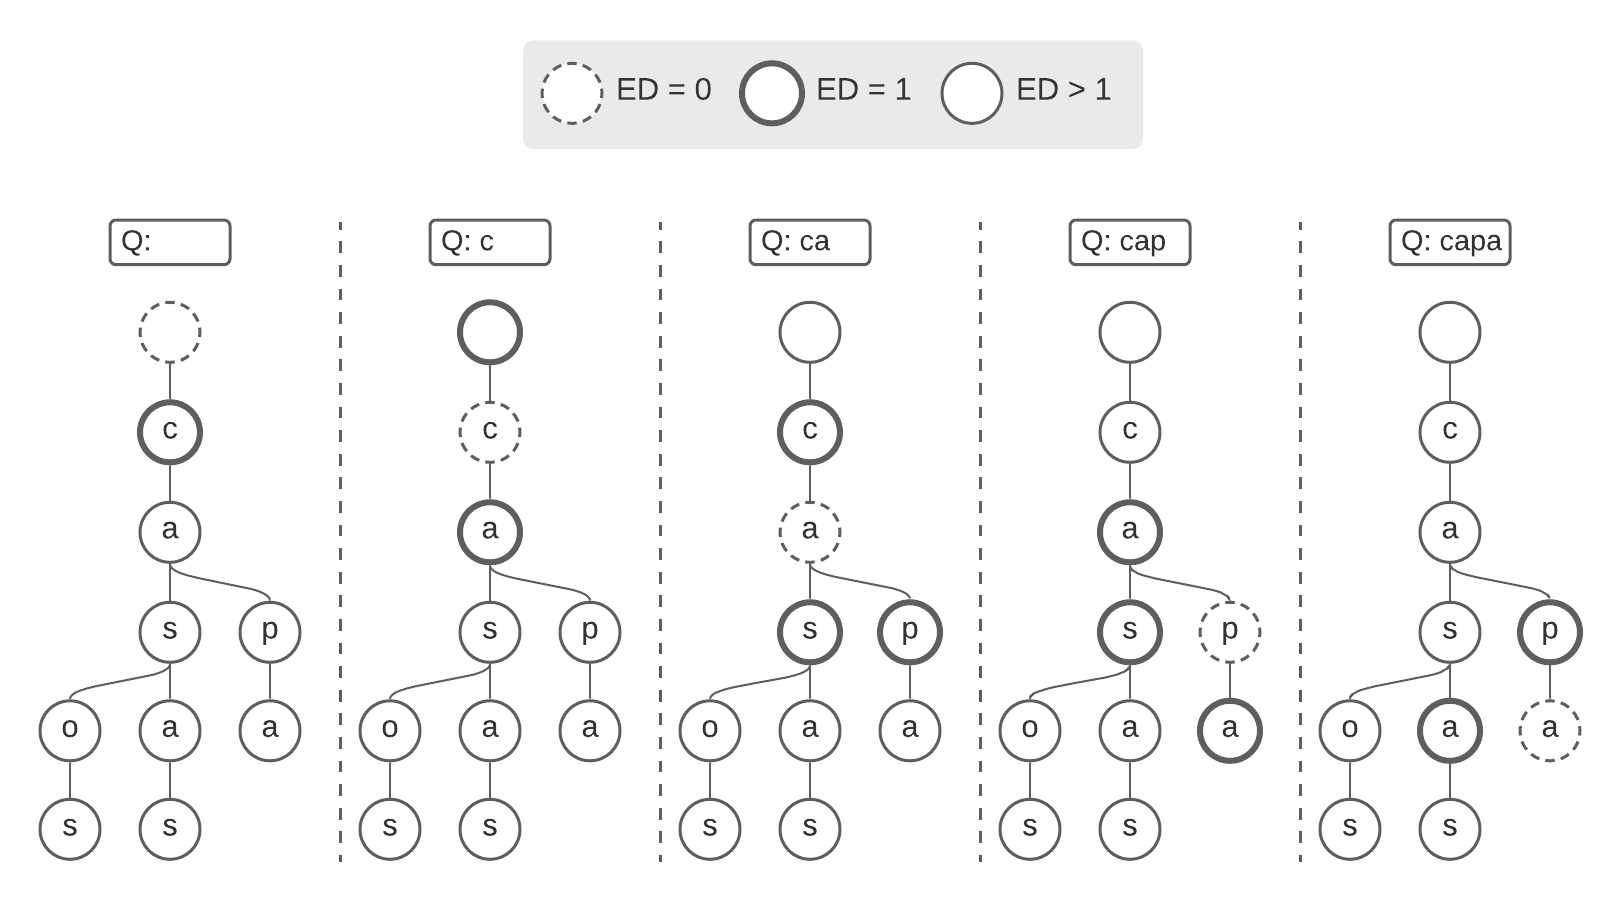
\includegraphics[width=1\textwidth]{figures/trie_active_nodes_example.png}
    \caption{Exemplo de ativação de nós da \textit{Trie} durante o processamento do prefixo de consulta $p = ``capa"$, considerando $\tau = 1$. }
    \label{fig:active_nodes_example}
\end{figure}

Um nó é considerado ativo quando a distância de edição entre seu prefixo e o prefixo consultado é menor ou igual ao limite $\tau$ considerado. O conjunto de nós ativos para um prefixo de consulta $p$ é definido como $V_{p} = \{p_{d} | p_{d} \in P(D) \land ed(p_{d}, p) \leq \tau \}$, onde $P(D)$ é o conjunto de prefixos da base de dados $D$, $p_{d}$ é um prefixo pertencente a $P(D)$ e $p$ é o prefixo de consulta. 

A Figura~\ref{fig:active_nodes_example} demonstra um exemplo de ativação de nós do índice \textit{Trie} à medida que o processamento do prefixo de consulta ``capa'' vai ocorrendo. O limiar de erros tolerados é $\tau = 1$. No início do processamento, considera-se o termo consultado como sendo uma cadeia de caracteres vazia, cujo valor é representado por $\epsilon$. A partir disso, é necessário ativar todos os nós (prefixos) da \textit{Trie} cujos prefixos possam ser transformados no prefixo de consulta, o qual é $\epsilon$ inicialmente. Portanto, os prefixos $\epsilon$ (representado pelo nó raiz da \textit{Trie}) e ``c'' são considerados nós ativos, pois $ed(\epsilon, \epsilon) = 0$ (círculo tracejado) e $ed(``l", \epsilon) = 1$ (círculo de borda grossa). Após isso, o prefixo consultado passa a ser primeira letra de ``capa'', ``c''. Então, é necessário analisar os nós já ativos (e seus respectivos filhos) do prefixo consultado anteriormente para computar os novos nós ativos para ``c''. A análise de cada nó ativo termina quando se encontra um prefixo fora do limiar $\tau$. Os novos nós ativos computados são $\epsilon$, ``c'' e ``ca'', porque $ed(\epsilon, ``c"") = 1$, $ed(``c", ``c"") = 0$ e $ed(``ca", ``c"") = 1$. Todos os outros prefixos além desse possuem distância de edição maior que o limite $\tau = 1$, portanto não são considerados nós ativos. Quando o prefixo de consulta passa a ser ``ca'', o nó raiz já não é mais um nó ativo, pois $ed(\epsilon, ``ca") = 2$, o nó ``c'' continua como nó ativo porém agora com uma distância igual a $1$ em relação a ``ca'', e dois novos nós são ativos, sendo eles  ``cas'' e ``cap'', ambos com distância igual a $1$ também. Esse algoritmo é repetido até chegar no final do prefixo de consulta ``capa'', cujos nós ativos são ``casa'' e ``capa''. O objetivo de computar nós ativos é o de utilizá-los para identificar itens similares ao prefixo consultado.

\subsection{ICAN}

O algoritmo proposto por \cite{ji2009efficient} denomina-se ``Computando Nós Ativos Incrementalmente'' (\textit{Incrementally Computing Active Nodes } -- ICAN). Considerando uma consulta de prefixo $p$ com apenas uma palavra-chave, para processar os nós ativos de forma eficiente é necessário computar e armazenar um conjunto de tuplas $\Phi_{p} = \{ \langle n, \xi_{n} \rangle \}$ tal que (1) cada $n$ é um nó ativo em relação à $p$ com $\xi_{n} = ed(n, p) \leq \tau)$ e (2) quaisquer nós ativos de $p$ estão presentes em $\Phi_{p}$, que é o \textit{conjunto de nós ativos de p} \citep{ji2009efficient}. Quando o usuário digita mais um caractere $p + 1$ após ter digitado $p$, o conjunto $\Phi_{p}$ de nós ativos de $p$ pode ser usado para computar o conjunto $\Phi_{p + 1}$ de nós ativos da nova consulta.

\subsubsection{Descrição do Algoritmo}

\begin{figure}[ht]
    \centering
    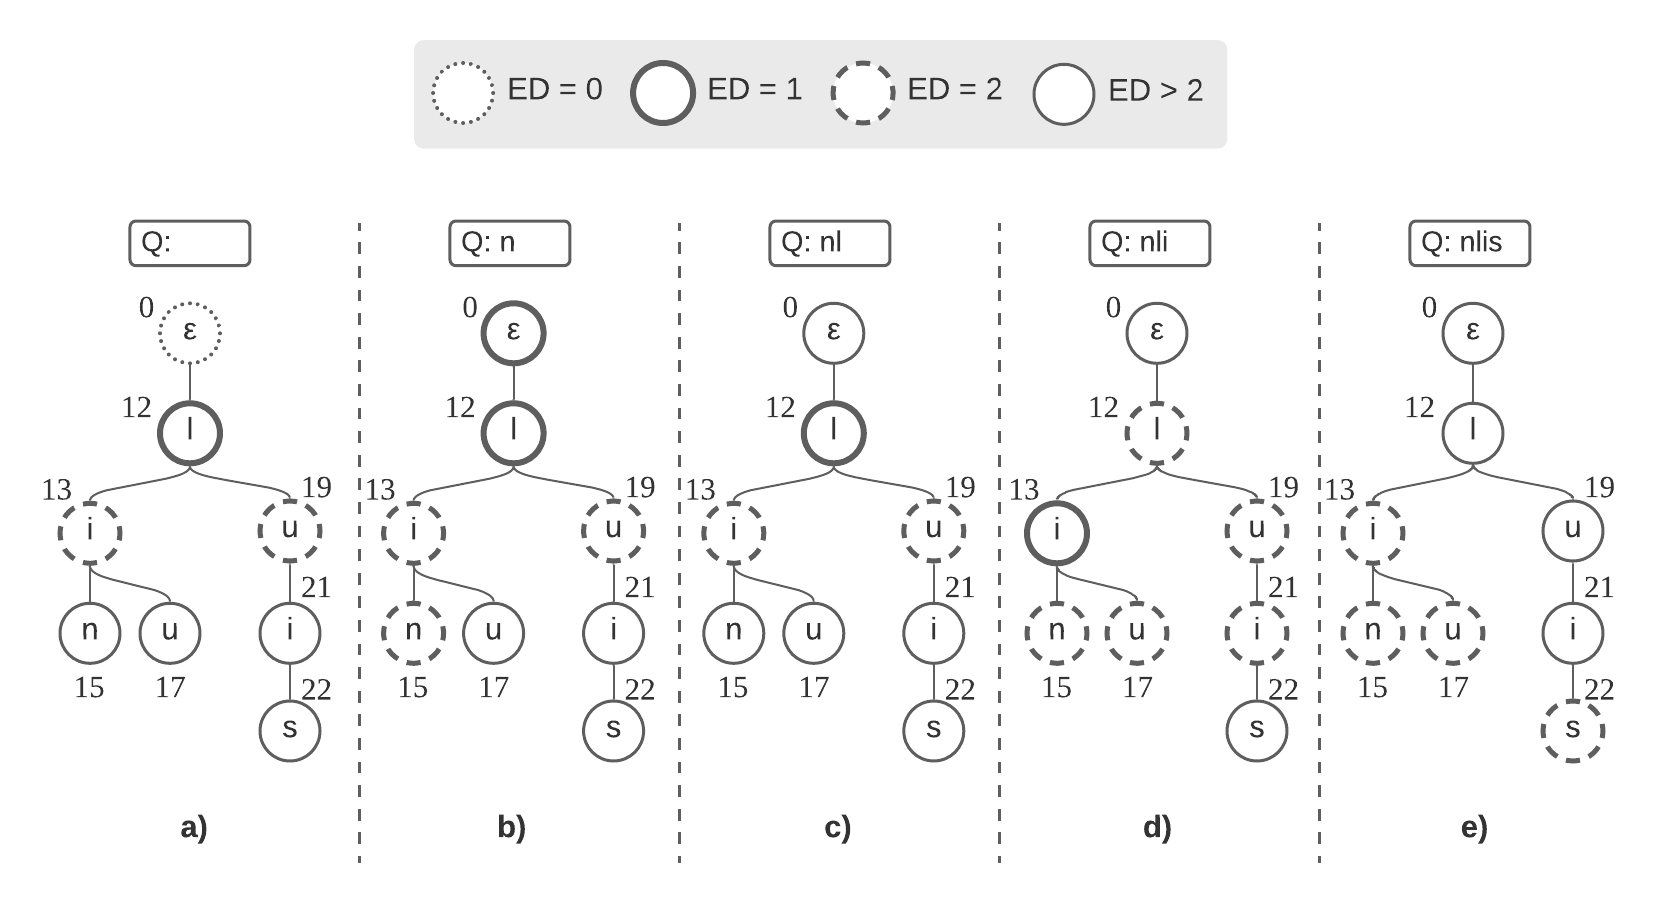
\includegraphics[width=1\textwidth]{figures/ican_example.png}
    \caption{Busca aproximada pelo prefixo de consulta ``nlis'' em uma \textit{Trie}, considerando o limiar de distância de edição $\tau = 2$. \textbf{(a)} Inicialização; \textbf{(b)} consulta por ``n''; \textbf{(c)} consulta por ``nl''; \textbf{(d)} consulta por ``nli''; \textbf{(e)} consulta por ``nlis'' }
    \label{fig:ican_example}
\end{figure}

Antes do usuário digitar qualquer caractere, o prefixo de consulta é considerado uma cadeia vazia $\epsilon$, o qual possui um conjunto de nós ativos $\Phi_{\epsilon}$ correspondente, que é inicializado como $\Phi_{\epsilon} = \{\langle n, \xi_{n} \rangle | \xi_{n} = |n| \leq \tau\}$. Esse conjunto inclui todos os nós $n$ da \textit{Trie} cujos prefixos correspondentes possuem um tamanho $|n|$ que é menor ou igual ao limiar $\tau$. No exemplo da Figura~\ref{fig:ican_example}, o primeiro passo é inicializar o conjunto $\Phi_{\epsilon} = \{ \langle n_{0}, 0\rangle, \langle n_{12}, 1\rangle,  \langle n_{13}, 2\rangle,  \langle n_{19}, 2\rangle \}$

\begin{figure}[ht]
    \centering
    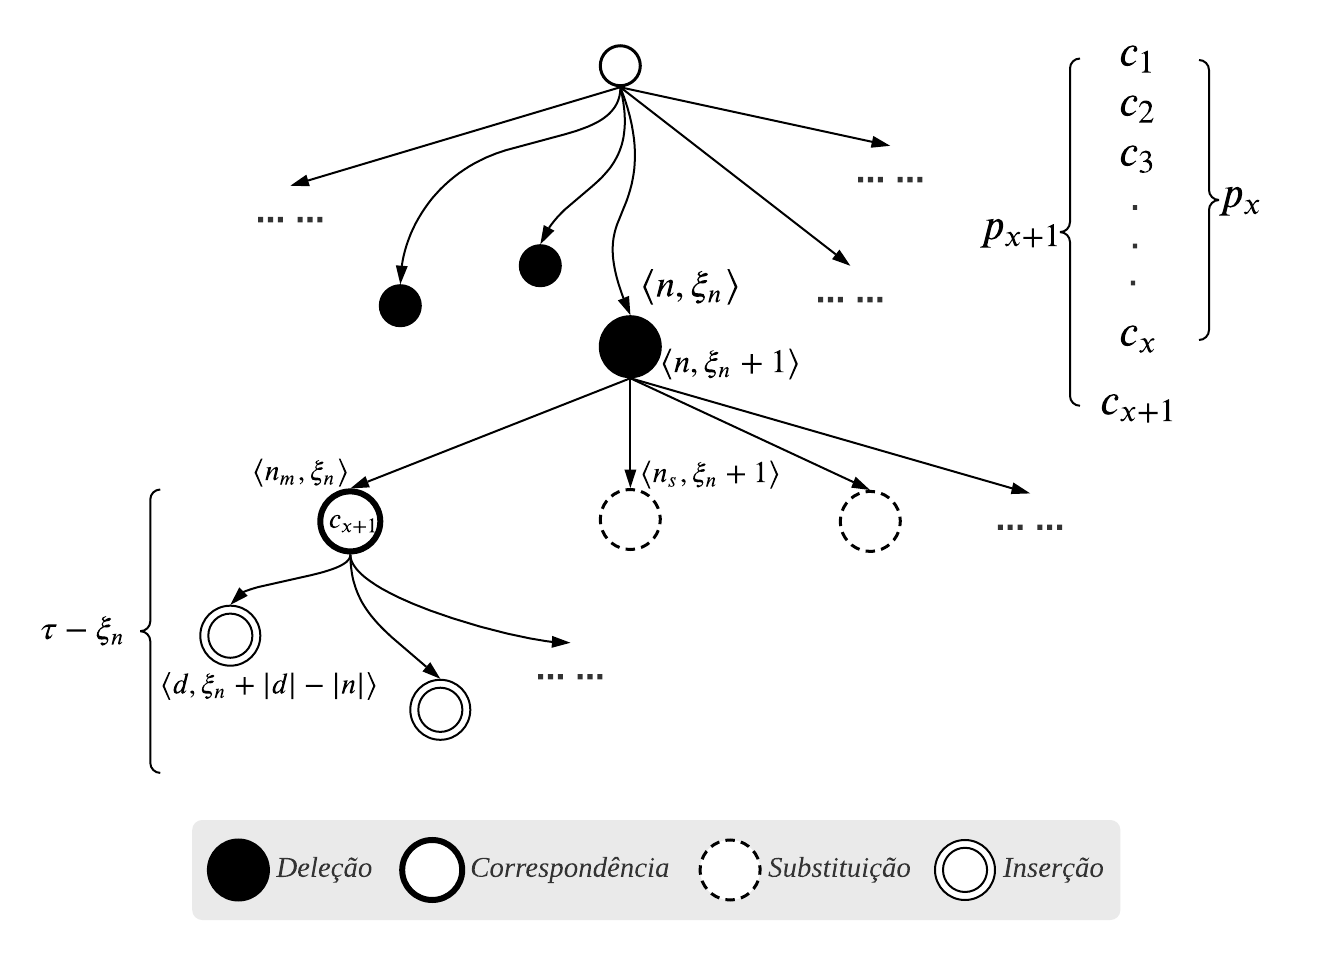
\includegraphics[width=1\textwidth]{figures/incrementally_computing_active_node_set.png}
    \caption{Computação incremental do conjunto de nós ativos $\Phi_{p_{x+1}}$ a partir do conjunto $\Phi{p_{x}}.$ O nó ativo de $\Phi{p_{x+1}}$ considerado é $\langle n, \xi_{n} \rangle$.}
    \label{fig:incrementally_computing_active_node_set}
\end{figure}

Suponhamos que após o usuário digitar o prefixo de consulta $p_{x} = c_{1}c_{2}...c_{x}$, o conjunto de nós ativos $\Phi_{p_{x}}$ para $p_{x}$ é computado. Quando o usuário digitar um novo caractere $c_{x+1}$ e formar um novo prefixo de consulta $p_{x+1}$, o algoritmo computa o conjunto $\Phi_{p_{x+1}}$ para $p_{x+1}$ a partir de $\Phi{p_{x}}$ da seguinte maneira: inicialmente, inicializa-se $\Phi{p_{x+1}}$ como um conjunto vazio; então, para cada tupla $\langle n, \xi_{n} \rangle$ em $\Phi_{p_{x}}$, apenas os descendentes de $n$ são examinados como candidatos de nós ativos para $p_{x+1}$, como é ilustrado na Figura~\ref{fig:incrementally_computing_active_node_set}. Nesse processo, é preciso atentar para os seguintes casos:

\textit{Considerando o nó $n$}: Seja $n$ um nó ativo de $p_{x}$. É possível transformar $n$ para $p_{x+1}$ com $\xi_{n} + 1$ operações de edição ao realizar primeiro uma transformação de $n$ para $p_{x}$ (com $\xi_{n}$ operações) e então deletar o último caractere $c_{x+1}$. Se $\xi_{n} \leq \tau$, então adicionamos a tupla $\langle n, \xi_{n} + 1 \rangle$ em $\Phi_{x + 1}$. Considerando a tupla $\langle n_{0}, 0 \rangle \in \Phi_{\epsilon}$ no exemplo da Figura~\ref{fig:ican_example}, quando o usuário digita o primeiro caractere ``n'' adiciona-se $\langle n_{0}, 1 \rangle$ em $\Phi_{n}$, pois é possível realizar uma operação de deleção na letra ``n'' com distância de edição igual a $1$. É importante ressaltar que devido à igualdade $\Phi_{p_{x}} = \Phi_{c_{1}c_{2}..c_{x}}$, o símbolo $\Phi_{n}$ nesse contexto refere-se ao \textit{conjunto de nós ativos para o prefixo de consulta ``n''}, e não possui relação com a variável $n$ utilizada para representar nós da \textit{Trie} anteriormente.

\textit{Considerando os filhos do nó $n$}: Para cada filho $n_{c}$ de um nó $n$, há dois possíveis casos:

\textit{Caso 1}: O nó filho $n_{c}$ tem um caractere diferente de $c_{x+1}$. A Figura~\ref{fig:incrementally_computing_active_node_set} mostra um nó $n_{s}$, onde ``s'' refere-se à operação de \textit{substituição}. É possível transformar $n_{s}$ em $p_{x+1}$ com $\xi_{n} + 1$ operações ao transformar primeiro $n$ em $p_{x}$ (com $\xi_{n}$ operações) e então substituir o caractere de $n_{s}$ por $c_{x+1}$. Se $\xi_{n} + 1 \leq \tau$ então adiciona-se $\langle n_{s}, \xi_{n} + 1 \rangle$ em $\Phi_{p_{x+1}}$. Esse caso corresponde a substituir o caractere de $n_{s}$ por $c_{x+1}$. No exemplo da Figura~\ref{fig:ican_example}, consideremos o caso em que o usuário digita o primeiro caractere ``n''. Para $\langle n_{0}, 0 \rangle \in \Phi_{\epsilon}$, o nó $12$ é filho do nó $0$ e possui a letra ``l''. Uma vez que é possível aplicar uma operação de substituição de ``l'' por ``n'' com $1$ operação  edição, adiciona-se $\langle n_{12}, 1 \rangle$ em $\Phi_{n}$. 

\textit{Caso 2}: O nó filho $n_{c}$ possui um caractere que corresponde ao caractere $c_{x+1}$ (o caractere de $n_{c}$ é igual a $c_{x+1}$). A Figura~\ref{fig:incrementally_computing_active_node_set} mostra o nó $n_{m}$, onde ``m'' refere-se à operação de \textit{correspondência}. É possível transformar $n_{m}$ para $p_{x+1}$ com $\xi_{n}$ operações ao transformar primeiro $n$ em $p_{x}$ (com $\xi_{n}$ operações) e então igualando o caractere de $n_{m}$ com $c_{x+1}$. Adiciona-se $\langle n_{m}, \xi_{n} \rangle$ em $\Phi_{p_{x+1}}$. Adicionalmente, se $\xi_{n} < \tau$ então as seguintes operações também são necessárias: para cada descendente $d$ de $n_{m}$ que dista no máximo $\tau - \xi_{n}$ letras de $n_{m}$, é preciso adicionar $\langle d, \xi_{d} \rangle$ em $\Phi_{p_{x+1}}$, sendo $\xi_{d} = \xi_{n} + |d| - |n_{m}|$. No exemplo da Figura~\ref{fig:ican_example}, suponhamos que o usuário digite o primeiro caractere ``l''. Para $\langle n_{0}, 0 \rangle \in \Phi_{\epsilon}$, o nó $12$ é filho do nó $0$ e possui a letra ``l''. Uma vez que o caractere do nó $12$ corresponde ao caractere ``l'', $\langle n_{12}, 0 \rangle$ é adicionado em $\Phi_{l}$. Além disso, o nó $13$ é filho do nó $13$. Uma vez que é possível adicionar o caractere de $n_{13}$ (``i'') após o nó $12$ com $1$ operação de edição, adiciona-se $\langle n_{13}, 1 \rangle$ em $\Phi_{l}$.

Para manter apenas as distâncias de edição mínimas no conjunto de nós ativos, durante a computação de $\Phi_{p_{x+1}}$, toda vez que se deseja adicionar uma tupla $\langle v, \xi_{1} \rangle$ ao conjunto é possível que o mesmo já contenha a tupla $\langle v, \xi_{2} \rangle$ para o mesmo nó $v$ no conjunto. Então, se $\xi_{1} \geq \xi_{2}$ a nova tupla não é adicionada. Se $\xi_{1} < \xi_{2}$, então a nova tupla substitui a original no conjunto. Ou seja, para um mesmo nó $v$ da \textit{Trie} no novo conjunto mantém-se apenas a sua menor distância de transformação para o prefixo de consulta $p_{x+1}$.

\subsection{ICPAN}

De acordo com o que foi dito na seção~\ref{sec:active_nodes}, o principal propósito de computar os nós ativos é usá-los para identificar itens similares ao prefixo consultado. Considerando o algoritmo ICAN, o conjunto de nós ativos final para o prefixo de consulta pode acabar sendo muito grande, o que aumenta o tempo de processamento. Diante desse problema \cite{li2011efficient} propuseram uma melhoria no algoritmo que consiste em podar nós ativos desnecessários, mas ainda mantendo a possibilidade de computar as respostas à consulta. As principais vantagens desse método são a redução do espaço de memória necessário para armazenar o conjunto de nós ativos, e também a redução do tempo de processamento da consulta, pois não é necessário examinar todos os nós ativos. 
Segue um exemplo de poda que reflete a intuição por trás desse método. Ainda considerando o exemplo da Figura~\ref{fig:incrementally_computing_active_node_set}, seja ``nl'' prefixo consultado com um limiar $\tau = 2$, onde $\Phi_{nl} = \{ \langle n_{12}, 1\rangle, \langle n_{0}, 2\rangle,  \langle n_{13}, 2\rangle,  \langle n_{19}, 2\rangle \}$. No entanto, apesar de $n_{13}$ (``li'') e $n_{19}$ (``lu'') serem nós ativos, não é necessário mantê-los, pois é possível utilizar o nó ativo $n_{12}$ (``l'') para computar as palavras ``li'' e ``lu''. Ou seja, é necessário manter apenas o nó ativo ``l'' para computar o mesmo conjunto de itens similares ao prefixo ``nl'' consultado.

\subsubsection{Nós Pivô Ativos}
\label{sec:pivotal_active_nodes}

Seja $n$ um nó ativo de $p$. Se para qualquer transformação de $n$ para $p$ com $ed(n,p)$ operações a operação no último caractere de $n$ não for uma correspondência (caracteres iguais), e for possível deletar o último caractere de $n$, o nó $n$ não é mantido, e sim o seu nó pai. Assim, surge o conceito de \textit{nó pivô ativo} \citep{li2011efficient}.

Considerando novamente o prefixo ``nl'' no exemplo da Figura~\ref{fig:incrementally_computing_active_node_set}, sabe-se que ``l'' é um nó ativo, e que ``li'' e ``lu'' são nós ativos cuja distância de edição entre ``nl'' é igual a $2$, e seus últimos caracteres não correspondem aos caracteres do prefixo ``nl''. É possível derivar esses dois nós ativos a partir do nó ``l'' ao inserir os caracteres ``i'' e ``u'', respectivamente. Além disso, também é possível computar as palavras similares ``li'' e ``lu'' ao visitar os nós folhas que são descendentes de ``l''. Portanto, não é necessário manter esses dois nós ativos. Nesse exemplo, o nó ``l'' é chamado \textit{nó pivô ativo}, pois serve como ``pivô'' para computar outras palavras similares à consulta sem a necessidade de ativar mais nós. Para um prefixo de consulta $p$, um nó $n$ é um nó pivô ativo de $p$ em relação ao limiar de distância de edição $tau$, se e somente se $n$ for um nó ativo de $p$ e se existir uma transformação de $p$ em $n$ com $ed(n,p)$ operações de edição, e a operação no último caractere de $n$ for a de correspondência. Ou seja, a operação no último caractere de $n$ não é nem uma deleção $ed(n,p) \neq ed(n', p) + 1$ e nem uma substituição $ed(n,p) \neq ed(n', p') + 1$, onde $n'$ e $p'$ são respectivamente os prefixos de $n$ e $p$ que não contêm o último caractere. 

Para computar de forma eficiente os nós pivô ativos, \cite{li2011efficient} desenvolveram o algortimo ``Computando Nós Pivô Ativos Incrementalmente'' (\textit{Incrementally Computing Pivotal Active Nodes } -- ICPAN). Sendo $p_{x}$ um prefixo de consulta, o objetivo é computar e armazenar um conjunto de 4-uplas $\Psi_{p_{x}} = \{ \langle n, \xi_{n}^{p_{x}}, p_{i}, \xi_{n}^{p_{i}} \rangle \}$. Em cada 4-upla do conjunto, $n$ é um nó pivô ativo de $p_{x}$, e \textit{$p_{i}$ é um prefixo de $p_{x}$ cujos últimos caracteres são iguais aos últimos caracteres de $n$}. Se esse prefixo não existir, então $p_{i} = \epsilon$. Se houver mais de uma possibilidade para $p_{i}$, então seleciona-se aquele com o menor número de caracteres. O quarto elemento da tupla, $\xi_{n}^{p_{i}} \leq \tau$ é a distância de dição entre o nó $n$ e o prefixo $p_{i}$ com operações de correspondência entre os últimos caracteres de $n$ e $p_{i}$. Já o segundo elemento da tupla, $\xi_{n}^{p_{x}} \leq \tau$ é a distância de edição entre nó $n$ e o prefixo de consulta $p_{x}$, obtida transformando primeiro $n$ em $p_{i}$, e então inserindo os caracteres restantes da diferença entre $p_{x}$ e $p_{i}$. A partir disso, deriva-se a igualdade $\xi_{n}^{p_{x}}=\xi_{n}^{p_{i}} + |p_{x}|-|p_{i}|$.

\subsubsection{Descrição do Algoritmo}
\label{sec:icpan_algorithm_description}

Antes do usuário digitar qualquer caractere, o prefixo de consulta é considerado uma cadeia vazia $\epsilon$, e então seu conjunto de nós pivô ativos correspondente é inicializado como $\Psi_{\epsilon} = \{ \langle r, 0, \epsilon, 0 \rangle \}$, onde $r$ é o nó raiz, já que a raiz é o único nó pivô ativo para $\epsilon$ de acordo com as definições estabelecidas anteriormente. Considerando ainda o mesmo exemplo da Figura~\ref{fig:incrementally_computing_active_node_set}, no qual o usuário digita o prefixo de consulta ``nlis'' caractere a caractere, e o limiar de distância de edição é $\tau = 2$, o primeiro passo é inicializar o conjunto como $\Psi_{\epsilon} = \{ \langle n_{0}, 0, \epsilon, 0 \rangle \}$, sendo $n_{0}$ o nó raiz. 

\begin{figure}[ht]
    \centering
    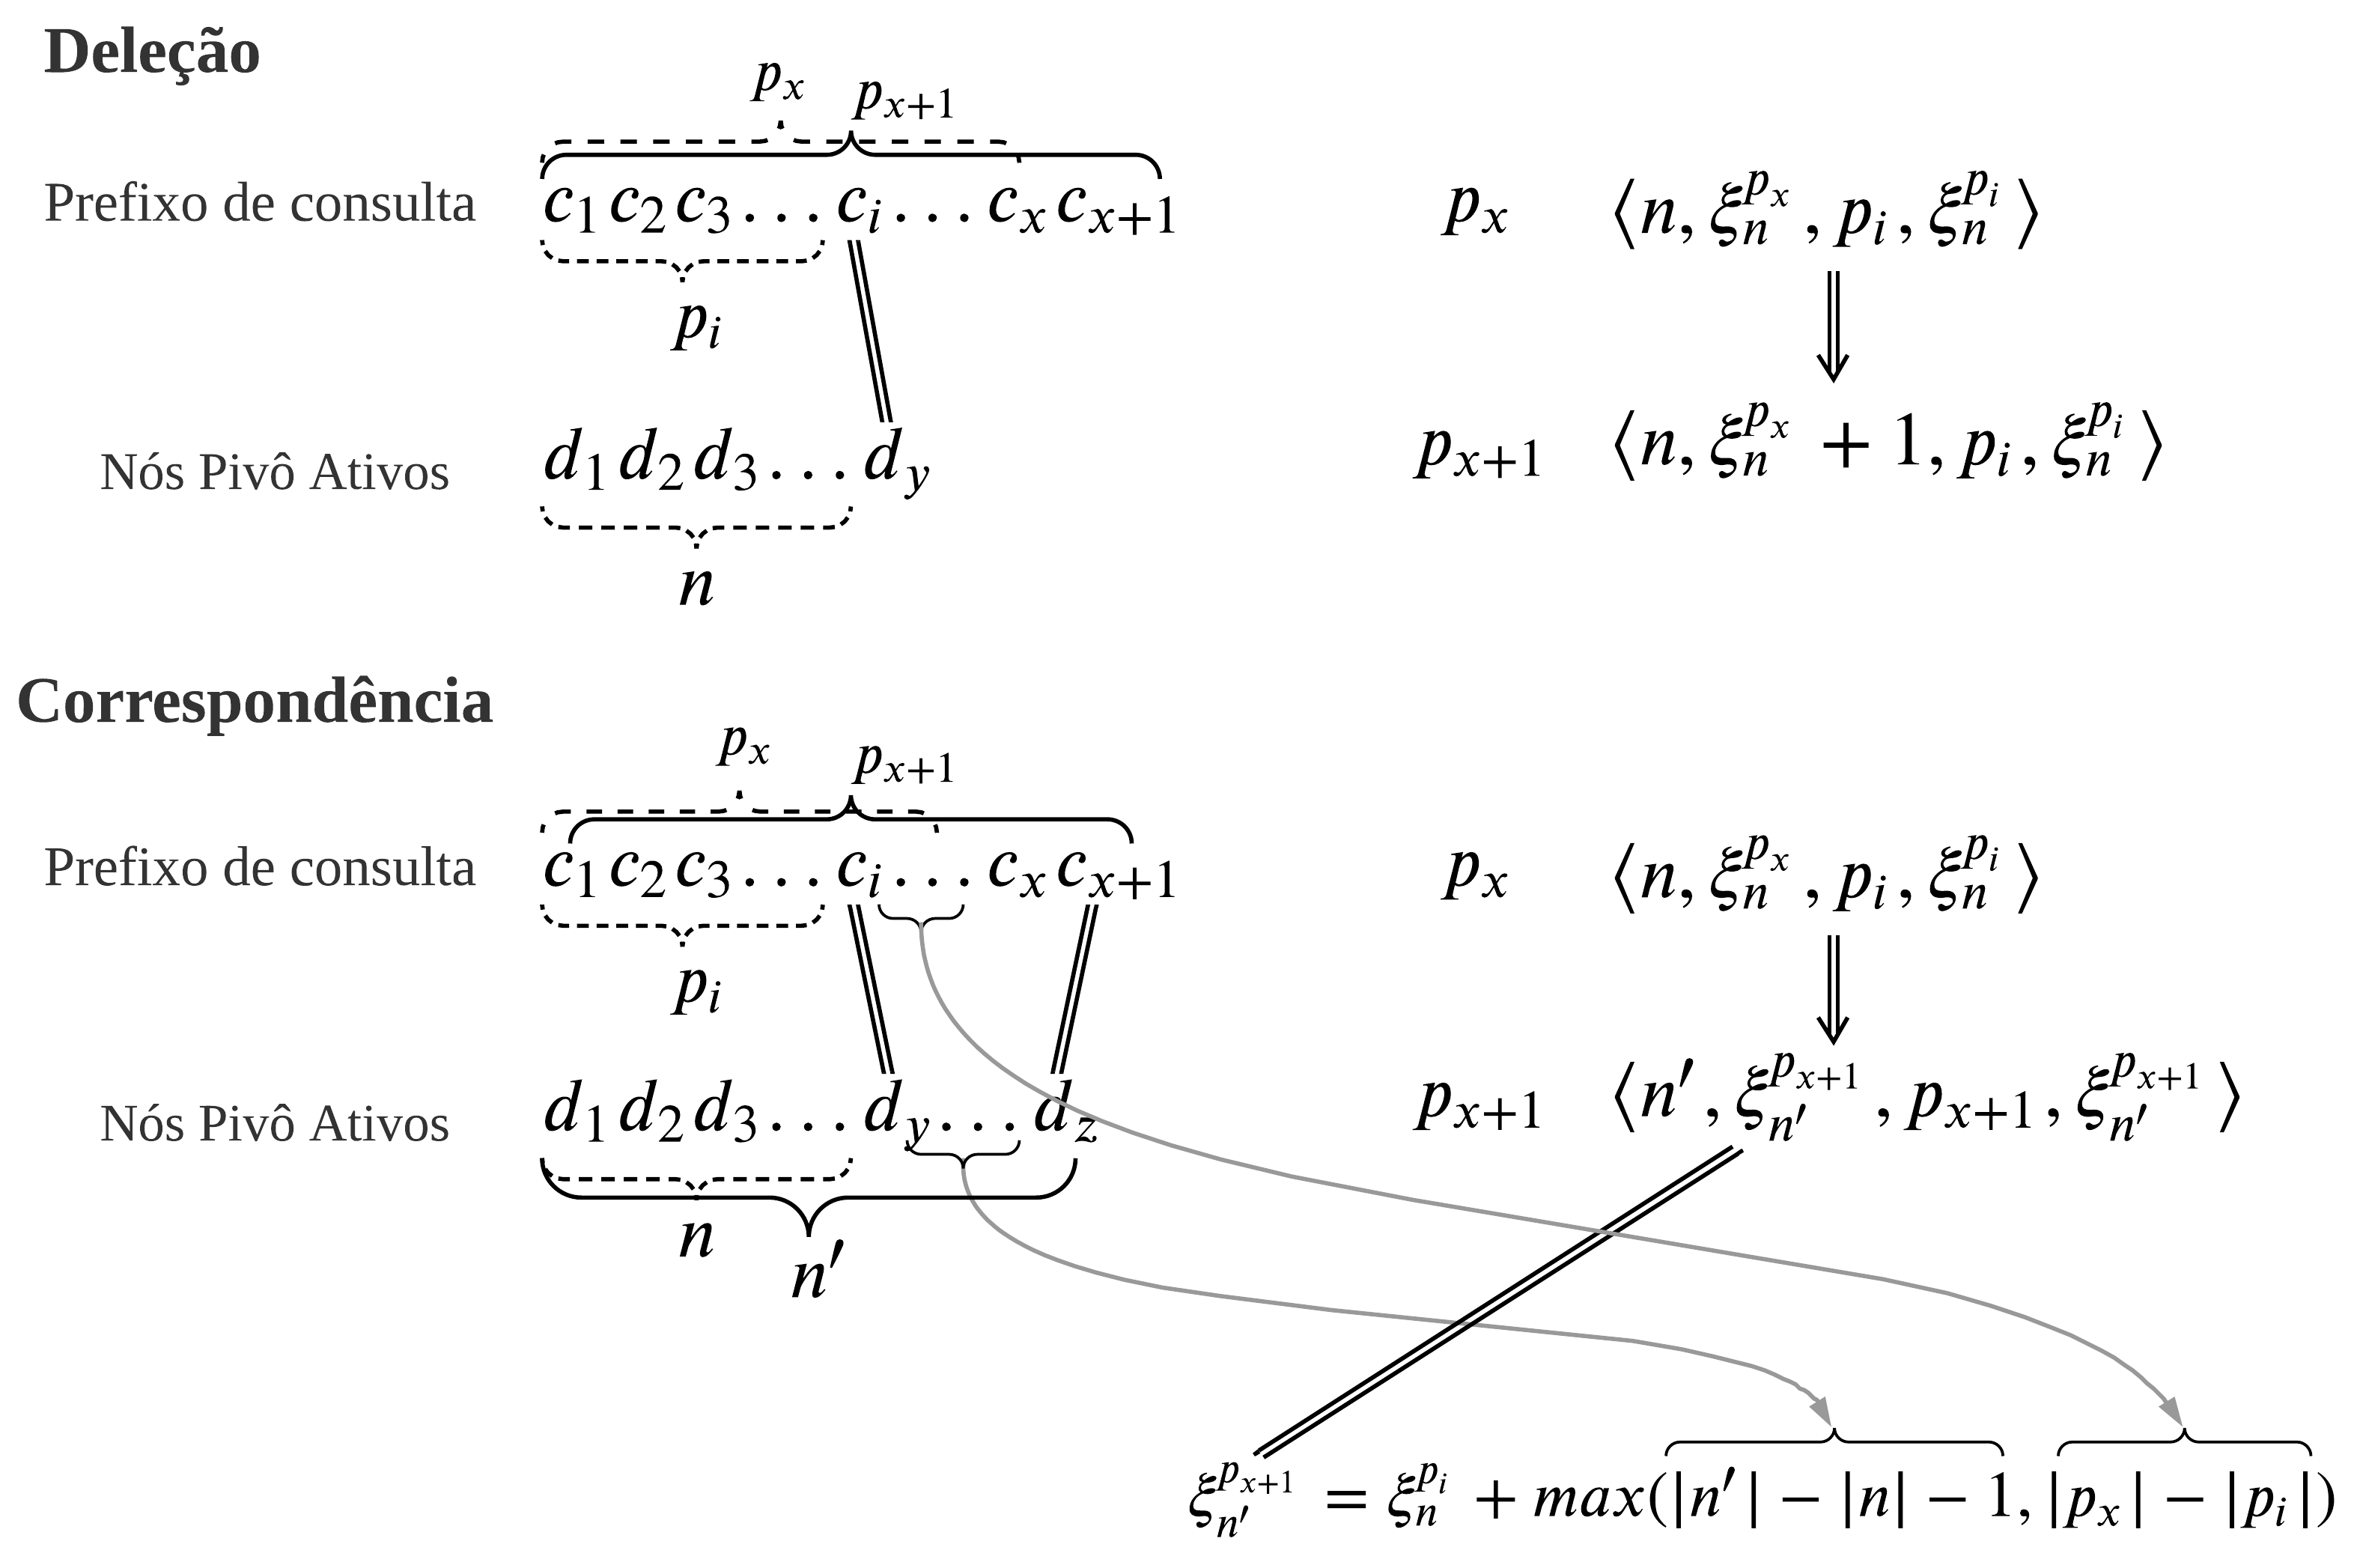
\includegraphics[width=1\textwidth]{figures/incrementally_computing_pivotal_nodes.png}
    \caption{Computação incremental de nós pivô ativos, sendo $c_{i} = d_{y}$ e $c_{x+1} = d_{z}$.}
    \label{fig:incrementally_computing_pivotal_nodes}
\end{figure}

Suponhamos que após o usuário digitar o prefixo de consulta $p_{x} = c_{1}c_{2}...c_{x}$, o conjunto de nós ativos $\Psi_{p_{x}}$ para $p_{x}$ é computado. Quando o usuário digitar um novo caractere $c_{x+1}$ e formar um novo prefixo de consulta $p_{x+1}$, o algoritmo computa o conjunto $\Psi_{p_{x+1}}$ para $p_{x+1}$ a partir de $\Psi{p_{x}}$ da seguinte maneira: inicialmente, inicializa-se $\Psi{p_{x+1}}$ como um conjunto vazio; então, para cada 4-upla $ \langle n, \xi_{n}^{p_{x}}, p_{i}, \xi_{n}^{p_{i}} \rangle$, apenas os descendentes de $n$ são examinados como candidatos de nós pivô ativos para $p_{x+1}$, como é ilustrado na Figura~\ref{fig:incrementally_computing_pivotal_nodes}. Nesse processo, é preciso atentar para os seguintes casos (todos os exemplos a seguir também consideram a árvore \textit{Trie} da Figura~\ref{fig:ican_example}):

\textit{Considerando o nó n}: Seja $n$ um nó pivô ativo de $p_{x}$. É possível transformar $n$ em $p_{x+1}$ com $\xi_{n}^{p_{x}} + 1$ operações de edição ao primeiro transformar $n$ em $p_{x}$ (com $\xi_{n}^{p_{x}}$ operações) e então deletar o último caractere $c_{x+1}$. Se $\xi_{n}^{p_{x}} + 1 \leq \tau$, então adiciona-se $\langle n, \xi_{n}^{p_{x}} + 1, p_{i}, \xi_{n}^{p_{i}} \rangle$ ao conjunto $\Psi_{p_{x+1}}$. Se o usuário digitar ``n'' por exemplo, uma vez que é possível realizar uma operação de deleção do caractere ``n'' com $1$ operação de edição, a partir da 4-upla $\langle n_{0}, 0, \epsilon, 0 \rangle \in \Psi_{\epsilon}$ é possível adicionar $\langle n_{0}, 1, \epsilon, 0 \rangle$ em $\Psi_{n}$.

\textit{Considerando os descendentes do nó n}: Consideremos os descendentes de $n$ \textit{que possuem o caractere $c_{x+1}$} e que não distem de $n$ mais do que $\tau - \xi_{n}^{p_{i}} + 1$ passos. Para esse descendente $n'$ nessa condição, é possível transformar $n'$ em $p_{x+1}$ com os seguintes passos: (1) transformar $n$ em $p_{i}$; (2) transformar os caracteres após $n$ e antes de $n'$ nos caracteres $c_{i+1}...c_{x}$; e (3) verificando a operação de correspondência do caractere $n'$ com $c_{x+1}$. Isso implica que é possível transformar $n'$ em $p_{x+1}$ com $\xi_{n'}^{p_{x+1}} = \xi_{n}^{p_{i}} + max(|n'| - |n| - 1, |p_{x}| - |p_{i}|)$ operações. Se $\xi_{n'}^{p_{x+1}} \leq \tau$, então adiciona-se $\langle n', \xi_{n'}^{p_{x+1}}, p_{x+1}, \xi_{n'}^{p_{x+1}} \rangle$ em $\Psi_{p_{x+1}}$. Por exemplo, se o usuário digitar o primeiro caractere ``n'' e considerando $\langle n_{0}, 0, \epsilon, 0 \rangle \in \Psi_{\epsilon}$, uma vez que o nó $n_{15}$(``lin'') corresponde a ``n'', então adiciona-se $\langle n_{15}, 2, ``lin", 2 \rangle$ em $\Psi_{n}$.

Semelhantemente ao ICAN, também é necessário manter a distância de edição mínima no conjunto de 4-uplas. Durante o processamento do novo conjunto $\Psi_{p_{x+1}}$, para um mesmo nó $n$, mantém-se somente a distância de edição entre o nó $n$ e o prefixo de consulta $p_{x+1}$. Toda vez que se deseja adicionar uma 4-upla $\langle n, \xi_{n}^{p_{x + 1}}, p_{i}, \xi_{n}^{p_{i}} \rangle$ ao conjunto é possível que o mesmo já contenha a 4-upla $\langle n, {\xi'}_{n}^{p_{x + 1}}, p_{j}, {\xi'}_{n}^{p_{j}} \rangle$ para o mesmo nó $n$ no conjunto. Se ${\xi'}_{n}^{p_{x+1}} > \xi_{n}^{p_{x+1}}$, então a nova 4-upla \textit{não é adicionada}. Se ${\xi'}_{n}^{p_{x+1}} = \xi_{n}^{p_{x+1}}$ e $|p_{j}| < |p_{i}|$, então a nova 4-upla substitui a 4-upla original (isso garante que apenas o prefixo com o menor número de caracteres seja mantido, como descrito em \ref{sec:pivotal_active_nodes}). Por fim, se ${\xi'}_{n}^{p_{x+1}} < \xi_{n}^{p_{x+1}}$, então a nova 4-upla \textit{substitui a original que já estava no conjunto}.

O ICPAN possui uma situação a mais para tratar em comparação ao ICAN: a remoção de nós ativos que não são pivôs. Para cada 4-upla $\langle n, \xi_{n}^{p_{x + 1}}, p_{i}, \xi_{n}^{p_{i}} \rangle$, \textbf{se $\mathbf{p_{i} \neq p_{x+1}}$}, então é feita uma verificação para cada nó ``ancestral'' $n_{a} \neq n$ de $n$. Se $\langle n_{a}, \xi_{n_{a}}^{p_{x + 1}}, p_{a}, \xi_{n_{a}}^{p_{a}} \rangle \in \Psi_{p_{x+1}}$ \textit{e} $\xi_{n_{a}}^{p_{a}} + max(|p_{x+1}| - |p_{a}|, |n| - |n_{a}|) < \xi_{n}^{p_{x+1}}$, então é preciso remover $\langle n, \xi_{n}^{p_{x + 1}}, p_{i}, \xi_{n}^{p_{i}} \rangle$ do conjunto. É necessário que isso aconteça pois nessas condições há uma transformação do nó $n$ para $p_{x+1}$ com uma distância de edição menor do que $\xi_{n}^{p_{x+1}}$ sem que haja correspondência no último caractere do nó $n$, ou seja, $n$ não é um nó pivô ativo do prefixo de consulta $p_{x+1}$.

Tanto o ICAN quanto o ICPAN produzem no final do processamento um conjunto de nós ativos. Os dois algoritmos consideram que cada nó folha $n_{folha}$ da árvore \textit{Trie} possui uma lista invertida $L$ de ``\textit{IDs}'' dos itens que possuem o prefixo referente ao nó $n_{folha}$. Então, para cada nó ativo do conjunto final obtido, obtem-se todos os nós folhas dentre seus descendentes. \textit{A lista de \textit{IDs} resultante das interseções entre as listas de todos esses nós folhas obtidos é a lista de itens similares ao prefixo consultado, ou seja, a resposta para o problema de CATE}.

\subsection{Busca em dois níveis}

Uma possível estratégia de busca em dois níveis para o problema de CATE consiste indexar somente parte dos itens da base de dados em uma árvore \textit{Trie}, e combinar um algoritmo de busca aproximada para essa estrutura (primeiro nível) com o algoritmo de busca sequencial apresentado na seção~\ref{sec:sequential_search} (segundo nível). Para isso, o prefixo de consulta também precisa ser divido em duas partes que são processadas por cada nível. Nessa abordagem, uma vez que os itens são indexados apenas parcialmente, o conjunto de nós ativos obtidos no final da execução do algoritmo do primeiro nível recebe uma nova função. Normalmente, tal conjunto é utilizado para computar os itens similares ao prefixo consultado, mas nessa abordagem de dois níveis, passa a ser usado como filtro para a busca sequencial do segundo nível, que é realizada somente nos itens referenciados por esses nós ativos.
 
\subsection{Busca binária com elementos repetidos na coleção}

Considerando a abordagem em dois níveis, neste trabalho analisamos a hipótese de que é possível utilizar não somente busca sequencial no segundo nível, mas também busca binária em alguns casos especiais, que são nós ativos com uma determinada característica explicada com mais detalhes na sessão~\ref{sec:metodo}. Nesses casos, é necessário realizar buscas binárias nas listas invertidas dos nós folha descendentes dos nós ativos.

O melhor algoritmo para busca em vetores ordenados é o de busca binária. Esse método requer que a coleção em que se fará a busca esteja ordenada. A busca binária padrão compara o valor buscado com o valor do elemento que se encontra no meio da coleção. Se eles não forem iguais, a metade da coleção na qual o valor buscado não pode ser encontrado é desconsiderada, e a busca continua na metade restante, considerando novamente o valor do elemento do meio. Esse processo se repete até que o valor seja encontrado. Se a busca terminar e a metade restante estiver vazia, a busca não encontrou o valor. A complexidade da busca binária é $O(\log n)$, enquanto a da busca sequencial é $O(n)$.

Porém, em algumas situações em que coleção possui elementos duplicados, pode ser necessário encontrar não um índice de um valor duplicado qualquer, mas o índice da primeira ocorrência do valor (limite inferior) juntamente com o índice da sua última ocorrência na coleção (limite superior). Para isso é necessário realizar primeiro uma busca binária especializada para encontrar o limite inferior, e depois realizar novamente outra busca binária própria para encontrar o limite superior. Após essas duas buscas, será obtido um intervalo $R = [limInferior, limSuperior]$ referente aos índices da coleção nos quais pode encontrar o valor duplicado que foi buscado. Nas buscas binárias por limite inferior e superior utilizadas no algoritmo~\ref{alg:2-level} da seção~\ref{sec:metodo}, quando o valor buscado não é encontrado consideramos os limites inferior e superior como sendo negativos, ou seja, $R = [-1, -1]$ por exemplo. 


\newpage
\thispagestyle{empty}
\mbox{}
\newpage

% ---------------------
% Método Proposto
% ---------------------
\chapter{Método proposto} 
\label{sec:metodo}

Neste capítulo estudaremos uma abordagem em dois níveis para a complementação automática de consulta tolerante a erros que usa o algoritmo \textit{ICPAN} no primeiro nível, e usa tanto pesquisa sequencial quanto binária no segundo nível. O primeiro nível serve como um filtro que seleciona candidatos à resposta para serem processados no segundo nível, responsável por determinar quais candidatos são qualificados como resposta final.

O intuito dessa abordagem é reduzir o uso de memória e ao mesmo tempo manter o desempenho quanto ao tempo de processamento da consulta. Os sistemas de busca podem se beneficiar dessa redução pois ela possibilita diminuir os custos com memória mantendo o mesmo conjunto de dados, ou então pode permitir o aumento do conjunto de dados sem que haja um grande impacto na quantidade de memória usada pelo método.

Seja $\mathcal{D}$ a base de dados considerada nos parágrafos a seguir, composta pelos seguintes itens: \textit{\{insects, integer, integral, integrity, intellect, intelligent, invest, invested, investigate, telepathic, telepathy, telephone, telephoto, teleport, teleprompter\}}. Atribuímos um valor de $id$ a cada item, partindo do número $0$, como é possível observar na tabela de itens da Figura~\ref{fig:index_structure}. A etapa de indexação considera que todos os itens estão ordenados em ordem lexicográfica crescente, e para que os exemplos fiquem mais simples cada item contém apenas uma palavra.
 
\section{Indexação} 
\label{sec:indexing}
Seja $w$ a cadeia de caracteres de um item, $|w|$ o tamanho da cadeia, e $w[i]$ uma indicação do $i$-ésimo caractere de $w$, com $i=1$ referindo-se ao primeiro caractere. A expressão $w[i..j]$ representa uma subcadeia de caracteres de $w$ começando na $i$-ésima posição e terminando na $j$-ésima. Consideramos também que se $j > |w|$, então $w[i..j] = w[i..|w|]$, e também que $w[i..]$ representa a subcadeia que começa no $i$-ésimo caractere, e termina no último caractere de $w$. Sendo assim, para $w = ``sapato"$, temos que $w[3..27] =  ``pato"$ e $w[4..] = ``ato''$, por exemplo.  

 
 \begin{figure} [ht]
    \centering
    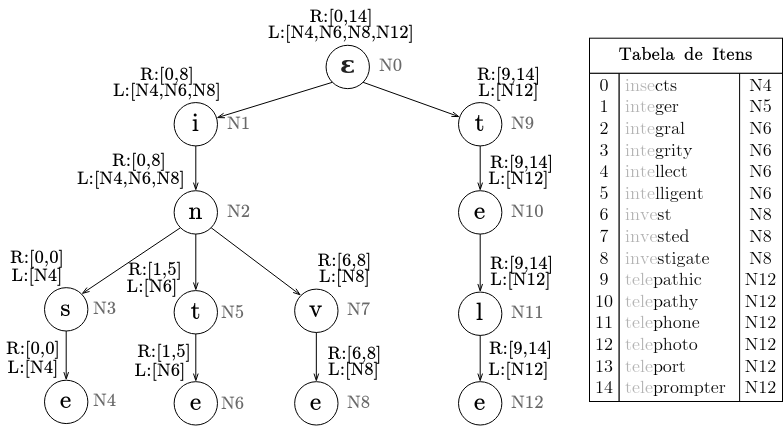
\includegraphics[width=0.94\textwidth]{figures/index-structure.png}
    \caption{Árvore \textit{Trie} com os prefixos de tamanho $\lambda = 4$ indexados, na qual cada nó possui intervalos $R$ de \textit{ids} e listas $L$ de nós folha dentre os seus descendentes.}
    \label{fig:index_structure}
\end{figure}

 
Como parte da implementação da estrutura proposta, indexamos as descrições textuais dos itens em uma árvore \textit{Trie} $\mathcal{T}$ mantida em memória. Seja também $\lambda$ a altura máxima permitida para $\mathcal{T}$, considerando que o nível do nó $\epsilon$ (nó $N0$ na Figura~\ref{fig:index_structure}) é igual a $0$. Dessa forma, o nó $N7$ tem altura igual a $3$, por exemplo. Para cada cadeia $w$ de um item inserimos em $\mathcal{T}$ apenas o prefixo $Prefixo_{\lambda}(w)$, onde $Prefixo_{\lambda}(s) = s[1..\lambda]$ é uma função que retorna os $\lambda$ primeiros caracteres da cadeia $s$ passada como parâmetro.

Cada nó $n$ em $\mathcal{T}$ contém um caractere $n.caractere$, um número de identificação $n.id$, e a sua altura $n.altura$ correspondente na árvore (sendo a altura do nó $\epsilon$ igual a 0). Também possui um intervalo $n.R = [menor, maior]$ no qual $menor$ e $maior$ representam respectivamente o menor e o maior $id$ dos itens em $\mathcal{T}$ que compartilham o mesmo prefixo $p_{n}$ obtido ao caminhar partindo do nó $\epsilon$ até $n$. Esse intervalo é análogo à lista invertida mencionada no fim da seção~\ref{sec:icpan_algorithm_description}. Para uma subárvore com raiz no nó $n$, todos os itens nessa subárvore irão compartilhar o mesmo prefixo $p_{n}$. Objetivando a simplicidade, iremos nos referir a $n$ pelo seu prefixo $p_{n}$ correspondente de forma intercambiável, assim como foi feito na seção~\ref{sec:trie}. 

Por fim, cada nó $n$ possui uma lista $n.L$ que contém todos os nós folha de sua subárvore. Quando o próprio $n$ é uma folha, não possui subárvore, então a lista conterá apenas o próprio $n$, ou seja, $n.L = [n.id]$.

A Figura~\ref{fig:index_structure} mostra uma \textit{Trie} $\mathcal{T}$ após a indexação dos $\lambda = 4$ primeiros caracteres de cada item em $\mathcal{D}$. Também mantém-se uma estrutura de dicionário $\mc{H}$, representada pela ``Tabela de Itens'', que mapeia o valor do \textit{id} de um item ao texto do restante da sua descrição, ou seja, $w[5..]$ (texto após o 4º caractere).

Essa estrutura é utilizada para reconstruir a descrição completa de um item a partir de qualquer nó de prefixo \textit{p}. Apesar da Figura~\ref{fig:index_structure} mostrar o texto completo de cada item na ``Tabela de Itens'', os $4$ primeiros caracteres em cinza claro são na verdade obtidos ao caminhar por $\mathcal{T}$. Para possibilitar essa reconstrução, também guardamos em $\mc{H}$ o $id$ do nó correspondente ao prefixo $Prefixo_{\lambda}(w)$ do item. Supondo por exemplo a reconstrução de ``\textit{investigate}'', com $id=7$ em $\mc{H}$, basta processar o prefixo $p$ do nó $N8$, que é \textit{p = ``inve''}, como mostra a Figura~\ref{fig:index_structure}, e então concatenar $p$ com ``\textit{stigate}'', que é o conteúdo presente em $\mc{H}$ para a chave $id=7$.

\begin{algorithm}[ht]
\caption{Construção de um índice \textit{Trie} $\mc{T}$ a partir de sugestões de consultas de uma base $\mc{D}$}\label{alg:dataset_indexing}
\begin{algorithmic}[1]
\Function{ConstruirIndiceTrie}{$\mc{D}, \mc{H}, \mc{T}$}
    \For{$Q \in \mc{D}$}
        \State $item.noPrefixo \leftarrow inserirPrefixo(\mc{T}, Prefixo_{\lambda}(Q.texto), Q.id)$
         \If{$|Q.texto| < \lambda$}
            \State $item.restante \leftarrow \epsilon$
         \Else{}
            \State $item.restante \leftarrow Q.texto[(\lambda + 1)..]$
         \EndIf
         
         \State $\mc{H}[Q.id] \leftarrow item$
    \EndFor
    \State $construirListasDeFolhas(\mc{T})$
\EndFunction
\end{algorithmic}
\end{algorithm}

O Algoritmo~\ref{alg:dataset_indexing} descreve a construção de um índice \textit{Trie} a partir de uma base de sugestões de consulta. Esse algoritmo tem como parâmetro: $\mc{D}, \mc{H}, \mc{T}$, os quais representam, respectivamente, a base de dados com as sugestões de consulta que serão indexadas, a estrutura de dicionário mencionada anteriormente, e a árvore \textit{Trie} ainda vazia. Esse algoritmo assume que os itens da base $\mc{D}$ estão em ordem lexicográfica crescente. O laço de repetição da linha 2 define o procedimento feito para cada sugestão de consulta $Q$ da base $\mc{D}$. Na linha 3, chama-se a função $inserirPrefixo$ (que será detalhada a seguir), a qual insere o prefixo $Prefixo_{\lambda}(Q.texto)$ (primeiros $\lambda$ caracteres do texto da sugestão de consulta) na \textit{Trie}, e retorna o nó da \textit{Trie} referente ao prefixo inserido. Então, esse nó é atribuído ao atributo $noPrefixo$ do $item$. Na linha 4, há uma condição para verificar se o tamanho do texto de $Q$ é menor que $\lambda$. Se for, então o atributo $restante$ do $item$ recebe o valor de texto vazio $\epsilon$, na linha 5. Senão, recebe o valor do restante do texto de $Q$ após o $\lambda$-ésimo caractere, na linha 7. Com o item já montado, associa-se a chave $Q.id$ com o $item$ no dicionário $\mc{H}$ na linha 8, e o laço de repetição segue para a próxima sugestão de consulta de $\mc{D}$, se houver. Após o termino do laço, chama-se a função $construirListasDeFolhas$ na linha 9. Essa função itera sobre cada nó $n$ da \textit{Trie}  $\mc{T}$, preenchendo as listas $n.L$ de cada nó, as quais contêm todos os nós folha com raiz em $n$.


\begin{algorithm}[H]
\caption{Inserção de um prefixo de sugestão de consulta em $\mc{T}$}\label{alg:append_prefix_trie}
\begin{algorithmic}[1]
\Function{inserirPrefixo}{$\mc{T}, prefixo, id$}
    \State $raiz \leftarrow obterRaiz(\mc{T})$d
    \State $n \leftarrow raiz$
    \State $raiz.R.maior = id$
    \For{$caractere \in prefixo$}
        \State $n \leftarrow n.inserirFilho(caractere, id)$
    \EndFor
    \State $n.marcadoFolha \leftarrow Verdadeiro$
    \State $n.L.inserir(id)$
    \State \textbf{return} $n$
\EndFunction
\end{algorithmic}
\end{algorithm}

O Algoritmo~\ref{alg:append_prefix_trie} descreve a inserção de um prefixo de sugestão de consulta (o qual pode na verdade ser a consulta inteira). Esse algoritmo tem como parâmetro: $\mc{T}, prefixo, id$, os quais representam a árvore \textit{Trie}, o prefixo de sugestão de consulta, e a identificação numérica da consulta, respectivamente. Na linha 4, atualiza-se o valor $maior$ do intervalo $raiz.R = [menor, maior]$ para ser igual ao $id$ da sugestão de consulta que está sendo inserida. Então, cada caractere do $prefixo$ (linha 5) é inserido na \textit{Trie} um a um na (linha 6). A cada inserção, o nó $n$ é atualizado com último nó que foi inserido ou apenas percorrido (caso todo o caminho já exista na árvore). Após essas inserções, na linha 8 o nó $n$ é marcado como folha. Por fim, o $id$ da sugestão de consulta é inserido na lista $L$ do nó $n$ na linha 9 e a função retorna $n$ na linha 10. 

\section{Algoritmo geral da abordagem em dois níveis}
\label{sec:general_two_level_algorithm}
% Esta premissa descrita a seguir não é 100% correta. Percebi no dia 26-05-2021 enquanto escrevia aqui que, com a implementação do conjunto de folhas virtuais, é possível computar nós ativos para os lambda+tau primeiros caracteres de p, ou para p inteiro caso |p| <= lambda + tau. Creio que vale a pena explorar essa premissa melhorada para a publicação do artigo.
Como descrito na seção~\ref{sec:indexing}, somente os $\lambda$ primeiros caracteres de cada sugestão de consulta da base são indexados na \textit{Trie}. Então, devido a esse fato, temos a premissa de que somente os $\lambda$ primeiros caracteres de um prefixo de consulta $p$ devem ser considerados na computação do conjunto de nós ativos. Com tal conjunto computado, cada nó é visitado, e recupera-se sua lista de nós folha. Para cada uma das listas invertidas desses nós folha, é possível realizar a busca sequencial apresentada na seção~\ref{sec:sequential_search}. 

\begin{algorithm}[H]
\caption{Algoritmo geral do processamento em dois níveis}\label{alg:general_two_level}
\begin{algorithmic}[1]
\Function{processarConsultaDoisNiveis}{$\mc{T}, p, \tau$}
    \If{$|p| + \tau \leq \lambda$} \textbf{return} $MetodoCATE(\mc{T},p,\tau)$
    \EndIf
    \State $sugestoes \leftarrow \emptyset$
    \State $nosAtivos \leftarrow computarNosAtivos(\mc{T}, Prefixo_{\lambda}(p), \tau)$ \Comment{Primeiro Nível}
    \For{$n \in nosAtivos$} \Comment{Segundo Nível (até a linha 6)}
        \For{$n_{folha} \in n.L$}
            \State $sugestoes \leftarrow sugestoes \cup buscaSequencial(p, n_{folha}.R, \tau)$
        \EndFor
    \EndFor
    \State \textbf{return} $sugestoes$
\EndFunction
\end{algorithmic}
\end{algorithm}

O Algoritmo~\ref{alg:general_two_level} é uma representação geral da abordagem em dois níveis para o problema de CATE. Ele tem como parâmetros $\mc{T}, p$ e $\tau$, os quais representam um índice \textit{Trie}, um prefixo de consulta, e o limiar de erros de digitação, respectivamente. O algoritmo tem início na linha 2 com uma verificação da condição $|p| + \tau \leq \lambda$, ou seja, se o tamanho do prefixo de consulta mais o número de erros de digitação tolerados é menor do que a altura máxima do índice \textit{Trie}.
Quando essa condição é verdade é possível utilizar somente o algoritmo de CATE (representado pela função \textit{MetodoCATE}) para computar todos os resultados para $p$, sem a necessidade de ativar o segundo nível. O prefixo de consulta pode sofrer no máximo $\tau$ inserções como erros de digitação, e se esse tamanho máximo ($|p| + \tau$) estiver dentro do limite $\lambda$, os nós indexados na \textit{Trie} são o suficiente para responder à consulta. Essa lógica estará presente também nos Algoritmos \ref{alg:ip2l} e \ref{alg:ip2lb}, com o método ICPAN sendo executado.

Caso a condição seja falsa, o algoritmo segue com o processamento em dois níveis. O conjunto de resposta $sugestoes$ é iniciado como vazio na linha 3, o qual conterá no fim da execução as sugestões de consultas com prefixos similares a $p$ considerando uma diferença de distância de edição de no máximo $\tau$. Na linha 4, é executada a função $computarNosAtivos$, que computa o conjunto de nós ativos da \textit{Trie} $\mc{T}$ para o prefixo $Prefixo_{\lambda}(p) = p[1..\lambda]$ considerando o limiar $\tau$. O algoritmo utilizado para tal computação pode ser, em tese, qualquer um baseado em processamento de nós ativos de árvores \textit{Trie}, como por exemplo o ICAN, ICPAN, ou BEVA. O conjunto final de nós ativos é armazenado na variável $nosAtivos$. Essa etapa caracteriza o primeiro nível. 

A linha 5 caracteriza o início do processamento do segundo nível. Nela há um laço de repetição que itera sobre cada nó ativo do conjunto $nosAtivos$, e na linha 6, há outro laço que itera sobre cada nó folha com raiz em $n$. Então, na linha 7, a função $buscaSequencial$ determina quais dentre as sugestões de consultas referenciadas pelo intervalo $R$ de $n_{folha}$ são respostas válidas, e então essas sugestões são unidas com o conjunto final de respostas. O algoritmo dessa função é o descrito na seção~\ref{sec:sequential_search}. Por fim, na linha 8 o conjunto de respostas é retornado.



\section{Primeiro nível}
\label{sec:first-level}

O algoritmo de busca utilizado no primeiro nível será o ICPAN, proposto por Li et al \citep{li2011efficient}. Como descrito no capítulo~\ref{sec:ref_teorico} o ICPAN utiliza um algoritmo incremental que calcula os prefixos semelhantes a um prefixo consultado, tolerando uma quantidade de erros de digitação previamente definida como o limite de distancia de edição $\tau$. Uma característica desse algoritmo é a ``ativação'' de nós da \textit{Trie} que correspondem a um prefixo que pode ser obtido considerando erros no prefixo consultado.

Ao considerar a utilização do ICPAN no primeiro nível, é preciso atentar para dois pontos: (1) uma vez que o primeiro nível serve apenas como filtro para o processamento do segundo nível, o algoritmo computará nós (pivô) ativos referentes a prefixos semelhantes a uma parte $p[1..\lambda]$ de um prefixo de consulta $p$, e não semelhantes a $p$ por completo. Esse conjunto será referido como $\Psi_{p[1..\lambda]}$ daqui em diante; (2) uma premissa da concepção original desse algoritmo é que todo o texto da sugestão de consulta estará indexado na \textit{Trie}, o que não acontece na abordagem em dois níveis.

Dessa maneira, o propósito original de utilização dos nós ativos foi modificado. Alguns nós importantes para o processamento no segundo nível acabam sendo desativados durante o processamento incremental do ICPAN, e deixam de estar presentes em $\Psi_{p[1..\lambda]}$. A partir dessa situação observamos em nossa pesquisa que o conteúdo do conjunto $\Psi{p[1..\lambda]}$ resultante da computação original do ICPAN \textit{não é suficiente para resolver completamente o problema de CATE na abordagem em dois níveis}. 

\subsection{Conjunto de nós folha virtuais ativos}
\label{sec:virtual_leaves_node-set}

Devido ao problema de nós desativados mencionado acima, faz-se necessário um mecanismo que preserve esses nós ativos importantes para que eles também estejam no conjunto final de nós ativos de $p[1..\lambda]$. O mecanismo proposto neste trabalho para resolver esse problema consiste em computar, simultaneamente ao conjunto de nós ativos $\Psi$ do ICPAN, um conjunto $\psi$ de ``nós folha virtuais ativos'' auxiliar que manterá esses nós importantes que acabariam sendo desativados durante o processamento incremental dos nós ativos. 

Como foi descrito na seção~\ref{sec:icpan_algorithm_description}, a computação do conjunto de nós ativos para um prefixo de consulta $p = c_{1}c_{2}c_{3}...c_{n}$ ocorre de forma incremental: inicializa-se um conjunto com os nós ativos para a cadeia vazia $\epsilon$, representado por $\Psi_{\epsilon}$; então, quando o primeiro caractere $c_{1}$ de $p$ é processado, os nós de $\Psi_{\epsilon}$ e alguns de seus descendentes são examinados e, dependendo de algumas condições, são inseridos no conjunto de nós ativos para a cadeia de caracteres $c_{1}$, representado por $\Psi_{c_{1}}$; quando o caractere $c_{2}$ é processado, analogamente ao passo anterior os nós de $\Psi_{c_{1}}$ e alguns de seus descendentes são examinados para determinar se serão inseridos no conjunto de nós ativos para a cadeia de caracteres $c_{1}c_{2}$, representado por $\Psi_{c_{1}c_{2}}$. Esse processo continua até que se obtenha o conjunto $\Psi_{p} = \Psi_{c_{1}c_{2}c_{3}...c_{n}}$, o qual será chamado de ``conjunto final''. Os conjuntos gerados antes do final serão chamados ``conjuntos intermediários''.

Na abordagem de dois níveis proposta neste trabalho, em que apenas os $\lambda$ primeiros caracteres das sugestões de consulta são indexados, a computação de nós ativos ocorre somente até o conjunto intermediário $\Psi_{p_[1..\lambda]}$, ou seja, o conjunto de nós ativos para os $\lambda$ primeiros caracteres de $p$. No entanto, existem alguns nós em especial que só podem ser encontrados no conjunto final, quando o processo continua após o $\lambda$-ésimo caractere. Quando se processa somente $p[1..\lambda]$, esses nós em especial são inseridos em alguns dos conjuntos intermediários, como em $\Psi_{c_1c_2}$, mas já não permanecem mais a partir de $\Psi_{c_1c_2c_3}$ em diante, por exemplo, e também não estarão inclusos no conjunto $\Psi_{p[1..\lambda]}$, que é utilizado para o processamento do segundo nível. A consequência desse problema é que algumas sugestões de consulta que só poderiam ser obtidas através desses nós não são analisadas no segundo nível, e então o algoritmo em dois níveis proposto deixa de trazer todos os resultados que deveria. Uma vez que ainda há texto do prefixo de consulta após o $\lambda$-ésimo caractere para considerar no cálculo de distância de edição que irá determinar se uma sugestão deve ser sugerida, esses nós precisam ser mantidos de alguma forma para também serem analisados no segundo nível.

Denominamos esses nós que acabam ``se perdendo'' durante a computação do conjunto de nós ativos como ``nós folha virtuais ativos''. Seja $\Psi_{c_{x}}$ o conjunto de nós ativos para um prefixo de consulta $p_{x} = c_1c_2...c_{x}$ digitado anteriormente, $c_{x+1}$ um novo caractere digitado pelo usuário que resulta no novo prefixo de consulta $p_{x+1} = c_1c_2...c_{x}c_{x + 1}$. Diante disso, é necessário examinar cada nó de $\Psi_{c_{x}}$ e alguns de seus descendentes para computar o conjunto $\Psi_{c_{x + 1}}$. Um nó é considerado como folha virtual ativo se, logo após examiná-lo em $\Psi_{c_{x}}$, não ocorre nenhuma inserção ou atualização em $\Psi_{c_{x + 1}}$, pois não foi possível realizar nenhuma substituição ou inserção de acordo com as regras de manutenção de conjunto de nós ativos do ICPAN definidas na seção~\ref{sec:icpan_algorithm_description}. O nome ``nó folha virtual ativo'' se dá pelo fato de que esse nó ativo, mesmo não sendo um nó folha de fato na \textit{Trie}, não gera nenhuma atualização do conjunto $\Psi_{c_{x + 1}}$ e também não vai gerar atualizações nos próximos conjuntos (quando houver).

Para manter os nós folha virtuais ativos encontrados durante a computação dos conjuntos de nós ativos, nós projetamos uma modificação no algoritmo de manutenção dos nós ativos do ICPAN para manter também um conjunto $\psi$ de nós folha virtuais ativos, representada no Algoritmo~\ref{alg:compute_active_and_virtual_leaf_nodes}.

O algoritmo tem como entrada os parâmetros $\Psi_{p_x}, \psi$ e $\tau, c_{x+1}$, os quais representam, respectivamente, o conjunto de nós ativos já computado para o prefixo digitado anteriormente, o conjunto de nós folha virtuais ativos, o limite de tolerância de erros de digitação, e o novo caractere do prefixo de consulta a ser processado. Na linha 2 o conjunto de nós ativos para o prefixo atualmente processado é criado, inicializado como um conjunto vazio. Na linha 3, a variável $ativaFolhasVirtuais$ recebe o resultado de uma expressão booleana que verifica se o tamanho do prefixo atual é maior que a diferença entre o limite $\lambda$ de altura do primeiro nível e o limite de tolerância de erros $\tau$. 

O resultado dessa expressão controlará se o conjunto $\psi$ será atualizado ou não. Sem esse controle, o conjunto $\psi$ acabará armazenando uma quantidade muito grande de nós, o que prejudicará o desempenho de processamento do segundo nível. Se $\lambda = 5$ e $\tau = 3$ por exemplo, ao considerar qualquer prefixo da \textit{Trie} com tamanho igual a $5$, ao aplicar a operação de $\tau = 3$ deleções, a subcadeia resultante terá obrigatoriamente tamanho $\lambda - \tau = 2$. Então, a heurística de ativação do conjunto $\psi$ se baseia nesse limite de $\tau$ deleções. 

Na linha 4 define-se o laço de repetição de iteração sobre todas as tuplas de $\Psi_{p_x}$. Na linha 5 é chamada a função $processarNoComICPAN$, que analisa o nó ativo presente na $tupla$ e alguns de seus descendentes de acordo com o algoritmo ICPAN apresentadas na seção~\ref{sec:icpan_algorithm_description}, além de atualizar (ou não) o conjunto de nós ativos atual $\Psi_{p_{x+1}}$. Para possibilitar a atualização do conjunto $\psi$, foi necessário modificar essa função originalmente utilizada no método ICPAN, para que ela passasse a retornar um valor booleano indicando se houve alguma alteração no conjunto $\Psi_{p_{x+1}}$. Esse valor é atribuído à variável $gerouAtualizacao$. Na linha 6 verificamos se o nó da $tupla$ não gerou atualização no conjunto $\Psi_{p_{x+1}}$ e se o conjunto $\psi$ deve ser atualizado. Se a expressão for verdadeira, então o conjunto $\psi$ é atualizado na linha 7. Por fim,. na linha 8 retorna-se uma tupla contendo os conjuntos $\Psi_{p_{x+1}}, \psi$.

\begin{algorithm}[t]
\caption{Computação incremental de nós ativos e nós folha virtuais }\label{alg:compute_active_and_virtual_leaf_nodes}
\begin{algorithmic}[1]
\Function{computarNosAtivosIncrementalmente}{$\Psi_{p_x}, \psi, \tau, c_{x+1}$}
    \State $\Psi_{p_{x+1}} \leftarrow \emptyset$
    \State $ativaFolhasVirtuais \leftarrow |p_{x+1}| > (\lambda - \tau)$
    
    \For{$tupla \in \Psi_{p_x}$}
        \State $gerouAtualizacao \leftarrow processarNoComICPAN(tupla, c_{x+1}, \Psi_{p_{x+1}})$
        
        \If{$\neg{gerouAtualizacao} \land ativaFolhasVirtuais$}
            \State $\psi \leftarrow \psi \cup \{tupla\}$
        \EndIf
    \EndFor
    
    \State \textbf{return} $\Psi_{p_{x+1}}, \psi$
\EndFunction
\end{algorithmic}
\end{algorithm}

\subsection{Computação de nós ativos no primeiro nível}
\label{sec:first_level_active_node_set_computation}

% Seja $p$ um prefixo consultado pelo usuário. Considerando que $p[1..\lambda]$ é uma sub-cadeia de caracteres de $p$ que vai do 1º até o $\lambda$-ésimo caractere, e que $p[1..\lambda] = p$ se $|p| \leq \lambda$, nós processamos a subcadeia $p[1..\lambda]$ na linha $3$ com o algoritmo ICPAN caractere a caractere, de acordo com os passos do algoritmo descritos na seção~\ref{sec:second_level}. Após terminar essa etapa obtemos um conjunto $\Psi_{p[1..\lambda]} = \{ \langle n, \xi_{n}^{p[1..\lambda]}, p_{i}, \xi_{n}^{p_{i}} \rangle \}$ de \textit{nós pivô ativos de} $p[1..\lambda]$. Se $|p| \leq \lambda$ consideramos que $p$ é uma consulta ``comum'', e então realizamos o processamento caractere a caractere padrão do ICPAN para obter a resposta na linha $5$. No entanto, quando $|p| > \lambda$, é necessário dividir o processamento em dois níveis.

Com a implementação do conjunto de nós folha virtuais ativos estabelecida é possível seguir para a computação do conjunto de nós ativos do primeiro nível, os quais serão utilizados como filtro para o segundo nível, como descrito na seção~\ref{sec:general_two_level_algorithm}. Ao fim desse processo os conjuntos $\Psi_{p[1..\lambda]}$ e $\psi$ terão sido computados (para os $\lambda$ primeiros caracteres de um prefixo de consulta $p$), e a união $\Psi_{p_[1..\lambda]} \cup \psi$ determina o ``conjunto final'' $\mc{F}$ que será de fato utilizado no segundo nível. 

No entanto, uma consequência dessa união é que o conjunto $\mc{F}$ possuirá nós folha virtuais ativos que foram ativados com diferentes subcadeias de $p[1..\lambda]$. Isto é, sendo $\lambda=6$, $\mc{F}$ conterá alguns nós folha virtuais que foram ativados quando $p[1..4]$ foi processado e outros que foram ativados ao processar $p[1..5]$, por exemplo. Diante dessa situação, torna-se necessário armazenar mais uma informação nas tuplas que compõem os conjuntos de nós ativos para realizar a busca binária do método IP2LB proposto neste trabalho (a seção~\ref{sec:IP2LB} possui mais detalhes). 

As tuplas passarão a conter um elemento a mais, denominado $\delta_{n}$, cujo valor representa o índice do caractere de $p[1..\lambda]$ que estava sendo processado no momento em que o nó $n$ foi adicionado/atualizado nos conjuntos $\Psi$ ou $\psi$, ou seja, tanto os nós ativos comuns quanto os nós folha virtuais ativos passarão a possuir o $\delta$ em suas respectivas tuplas. Se por exemplo $\lambda=5$ e $p[1..\lambda]=``sapat"$, e um nó ativo foi adicionado ao conjunto $\Psi$ quando a subcadeia $p[1..3]=``sap"$ foi processada, então $\delta_{n}=3$ é inserido na tupla referente ao nó $n$.

\begin{algorithm}[H]
\caption{Computação de nós ativos para o primeiro nível}\label{alg:compute_first_level_nodes}
\begin{algorithmic}[1]
\Function{computarNosAtivos}{$\mc{T}, p, \tau$}
    \State $raiz \leftarrow obterRaiz(\mc{T})$
    \State $\Psi = \{ \langle raiz, 0, \epsilon, 0 \rangle \}$
    \State $\psi = \emptyset$
    
    \For{$caractere \in Prefixo_{\lambda}(p)$}
        \State $\Psi, \psi \leftarrow computarNosAtivosIncrementalmente(\Psi, \psi, \tau, caractere)$
    \EndFor
    \State $\mc{F} \leftarrow \Psi \cup \psi$
    \State \textbf{return} $\mc{F}$
\EndFunction
\end{algorithmic}
\end{algorithm}

O Algoritmo~\ref{alg:compute_first_level_nodes} descreve esse procedimento, e tem como parâmetros $\mc{T}, p$ e $\tau$ que representam, respectivamente, o índice \textit{Trie}, o prefixo de consulta, e o limiar de erros de edição tolerado. Na linha 2, o nó raiz da \textit{Trie} é obtido. Na linha 3, o conjunto de nós ativos é inicializado com o nó raiz. Nesse momento, esse conjunto representa o conjunto $\Psi_{\lambda}$ de nós ativos para a cadeia vazia de caracteres. Esse conjunto será sobrescrito algumas vezes no decorrer do algoritmo, e no fim será representará o conjunto $\Psi_{p[1..\lambda]}$ de nós ativos para $p[1..\lambda]$. Na linha 4 o conjunto $\psi$ de nós folha virtuais ativos é inicializado como vazio. Então, na linha 5 define-se um laço de repetição para iterar sobre os $\lambda$ primeiros caracteres de $p$. Na linha 6 é chamada a função $computarNosAtivosIncrementalmente$, a qual foi descrita anteriormente na seção~\ref{alg:compute_active_and_virtual_leaf_nodes}. Os conjuntos retornados pela função sobrescrevem as variáveis $\Psi$ e $\psi$. Já na linha 7 atribui-se a união entre o conjunto $\Psi$ de nós ativos (que nesse momento representa o conjunto $\Psi_{p[1..\lambda]}$) e o conjunto $\psi$ à $\mc{F}$, que é retornada pela função na linha 8 a seguir.




% \begin{algorithm}[ht]
% \caption{Complementação de consultas tolerante a erros em dois níveis}\label{alg:2-level}
% \begin{algorithmic}[1]
% \Function{processarConsulta}{$p$}
%     \State $resultados \gets \emptyset$
%     \State $\Psi_{p[1..\lambda]} \gets processarConsultaComICPAN(p[1..\lambda])$  \Comment{Nós pivô ativos para $p[1..\lambda]$}
%     \If{$|p| < \lambda$}
%         \State \textbf{return} $recuperarResultadosICPAN(\Psi_{p[1..\lambda]})$
%     \EndIf
%     \For{$\langle n, \xi_{n}^{p[1..\lambda]}, p_{i}, \xi_{n}^{p_{i}} \rangle \in \Psi_{p[1..\lambda]} $}
%         \If{$\xi_{n}^{p[1..\lambda]} < \tau$}
%             \For{$n_{folha} \in n.L$}
%                 \For{$itemId \in n_{folha}.R$}
%                     \If{$itemId \in resultados$}
%                         \State \textbf{continue}
%                     \EndIf
%                     \State $candidato \gets H[itemId].reconstruirTexto()$
%                     \State $distancia \gets levenshtein(candidato[1..|p|], p)$ 
%                     \If{$distancia \leq \tau$}
%                         \State $resultados \gets resultados \cup \{ itemId \}$
%                     \EndIf
                    
%                 \EndFor
%             \EndFor
%         \Else
%             \For{$n_{folha} \in n.L$}
%                 \State $p' \gets p[\lambda+1+ (n.altura - |p_{i}|)..|p|]$
%                 \State $limInferior \gets buscaBinariaLimInf(p', n_{folha}.R, n.altura)$
%                 \State $limSuperior \gets buscaBinariaLimSup(p', n_{folha}.R, n.altura)$
                
%                 \If{$limInferior \ge 0$ \textbf{and} $limSuperior \ge 0$}
%                     \State $i \gets 0$
%                     \While{$i + limInferior \le limSuperior$}
%                         \State $resultados \gets resultados \cup \{ leaf.ids[limInferior + i] \} $
%                         \State $i \gets i + 1$
%                     \EndWhile
%                 \EndIf
%             \EndFor
%         \EndIf
%     \EndFor
%     \State \textbf{return} $resultados$ 
% \EndFunction
% \end{algorithmic}
% \end{algorithm}

% \newpage
\section{Segundo nível}
\label{sec:second_level}

Quando o conjunto final de nós ativos $\mc{F} = \Psi_{p[1..\lambda]} \cup \psi$ é computado para $p[1..\lambda]$ no primeiro nível, é preciso iniciar a etapa do segundo nível. Como dito anteriormente, cada nó $n$ pertencente a esse conjunto possui uma lista $L$ de nós folha, da qual cada nó $n_{folha}$ tem um intervalo $R$ que contém o menor e maior $id$ das sugestões de consulta que começam com o prefixo formado ao percorrer o caminho da raiz até $n_{folha}$. A etapa do segundo nível consiste em, para todas as sugestões de consulta referenciadas por todos esses nós folha, determinar quais delas possuem um prefixo similar à $p$ com no máximo $\tau$ erros de edição. 

\section{Utilizando somente busca sequencial} 
\label{sec:IP2L}

Para atingir esse objetivo, uma forma é realizar uma busca sequencial dentre essas sugestões de acordo com o algoritmo descrito na seção~\ref{sec:sequential_search}. Seja $n$ um dos nós presentes no conjunto $\mc{F}$, $n_{folha}$ um dos nós folha presentes em $n.L$. O intervalo $n_{folha}.R = [minimo, maximo]$ representa uma lista de $ids$ do dicionário $\mc{H}$ de sugestões indexadas. Ao aplicar nessa lista o algoritmo de busca sequencial descrito na seção~\ref{sec:sequential_search}, determinaremos quais das sugestões que começam com o prefixo $n_{folha}$ são similares ao prefixo de consulta $p$ considerando $\tau$ erros de digitação. Essa busca sequencial é realizada em todos os outros nós folhas de $n$. Além disso, esse procedimento que é realizado para $n$ também é executado para todos os outros nós em $\mc{F}$. Desse modo, obtém-se todos as sugestões de consulta similares à $p$, a resposta do problema de CATE.

Na configuração de dois níveis proposta neste trabalho é possível realizar uma otimização nos cálculos de distância de edição com matrizes de \textit{Levenshtein} para a acelerar a execução da busca sequencial. Sendo $n$ um nó ativo qualquer de $\mc{F}$, obviamente todas as sugestões que podem ser obtidas a partir desse nó começarão com o prefixo $n$. A consequência disso é que todas as matrizes de \textit{Levenhstein} calculada para determinar a similaridade entre $p$ e uma sugestão qualquer com o prefixo $n$ conterão um conjunto de linhas em comum (especificamente, as $|n|+1$ primeiras linhas). É redundante computar essas $|n|+1$ linhas em cada verificação entre $p$ e uma sugestão com prefixo $n$ realizada na busca sequencial para esse nó. 

Dessa forma, é possível eliminar essa redundância ao computar a linha de número $|n|+1$ da matriz gerada no cálculo de $ed(n,p)$ (os caracteres de $p$ ficam nas colunas da matriz) antes de iniciar a busca sequencial. Se algum dos valores da última coluna da matriz de $ed(n,p)$ for menor ou igual a $\tau$, todas as sugestões com prefixo $n$ podem automaticamente fazer parte do conjunto de resposta para o problema. Por fim, todos os cálculos de matrizes de \textit{Levenhstein} para as sugestões com o prefixo $n$ podem iniciar a partir dessa linha da matriz previamente computada. Denominamos esse método em dois níveis como ``IP2L'' (\textbf{I}C\textbf{P}AN \textbf{2}-\textit{\textbf{L}evel}), que está descrito no Algoritmo~\ref{alg:ip2l}.

\begin{algorithm}[H]
\caption{Complementação automática de consultas tolerante a erros com o IP2L}\label{alg:ip2l}
\begin{algorithmic}[1]
\Function{processarConsultaIP2L}{$\mc{T}, \mc{H} , p, \tau$}
    \If{$|p| + \tau \leq \lambda$} \textbf{return} $ICPAN(\mc{T},p,\tau)$
    \EndIf
    \State $sugestoes \leftarrow \emptyset$
    \State $\mc{F} \leftarrow computarNosAtivos(\mc{T}, Prefixo_{\lambda}(p), \tau)$ \Comment{Primeiro Nível}
    \For{$\langle n, \xi_{n}^{p[1..\lambda]}, p_{i}, \xi_{n}^{p_{i}} \rangle \in \mc{F}$} \Comment{Segundo Nível (até a linha 13)}
        \State $ultimaLinhaComum \leftarrow ultimaLinhaLevenhstein(n, p)$
        \For{$n_{folha} \in n.L$}
            \For{$id \in n_{folha}.R$}
                \State $sugestao \leftarrow recuperarTexto(\mc{H}[id])$
                \If{$ultimaLinhaComum[|p|] \leq \tau$}
                    \State $sugestoes \leftarrow sugestoes \cup \{ sugestao \}$
                    \State \textbf{continue}
                \EndIf
                \If{$similar(sugestao, p, ultimaLinhaComum, \tau)$}
                    \State $sugestoes \leftarrow sugestoes \cup \{ sugestao \}$
                \EndIf
            \EndFor
        \EndFor
    \EndFor
    \State \textbf{return} $sugestoes$
\EndFunction
\end{algorithmic}
\end{algorithm}

Esse algoritmo define a função $processarConsultaIP2L$, que tem como parâmetros $\mc{T}, \mc{H}, p$ e $\tau$, os quais representam, respectivamente, o índice \textit{Trie}, o dicionário ``Tabela de Itens'' mencionado na seção~\ref{sec:indexing}, o prefixo de consulta, e o limiar de erros de digitação. Na linha 2 há a verificação da condição para executar apenas o método ICPAN de acordo com o que foi mencionado na seção~\ref{sec:general_two_level_algorithm}. Na linha 3 inicializa-se o conjunto $sugestoes$ como vazio. Ao final da execução da função esse conjunto conterá todas as sugestões com prefixo similares $p$ considerando no máximo $\tau$ erros. Na linha 4, o conjunto $\mc{F}$ recebe o conjunto retornado pela execução da função $computarNosAtivos$ descrita no Algoritmo~\ref{alg:compute_first_level_nodes}. 

Então, na linha 5 define-se um laço de repetição que itera sobre cada 4-upla (nó pivô ativo) do conjunto $\mc{F}$. O primeiro passo do laço é calcular a última linha da matriz de \textit{Levenhstein} para $ed(n, p)$, com a função $ultimaLinhaLevenhstein$ na linha 6. O resultado será atribuído à variável $ultimaLinhaComum$, que será utilizada mais à frente para otimizar o processamento no segundo nível. 

Nesse contexto é importante ressaltar que $n$ é um nó da \textit{Trie} e não uma cadeia de caracteres. A função $ultimaLinhaLevenhstein$ internamente recupera o prefixo formado pelo caminho da raiz até o nó $n$ para utilizá-lo no cálculo da matriz de \textit{Levenhstein}. 

A linha 7 define um laço de repetição que itera sobre cada nó folha $n_{folha}$ de $n.L$, e a linha 8 a seguir também define outro laço no qual itera-se sobre cada valor de $id$ representado pelo intervalo $n_{folha}.R = [minimo, maximo]$. Na linha 9 recupera-se o texto completo da sugestão com a execução da função $recuperarTexto$, passando como parâmetro o item referenciado pela chave $id$ no dicionário $\mc{H}$. Então, a linha 10 define a condição para verificar se o valor da última coluna da $ultimaLinhaComum$ é menor ou igual a $\tau$. Se for, então a sugestão de consulta é adicionada ao conjunto $sugestoes$ na linha 11 e o laço de repetição segue para a próxima iteração. Essa função concatena o prefixo formado pelo caminho da raiz até o nó $\mc{H}[id].noPrefixo$ e o concatena com a cadeia $\mc{H}[id].restante$. A linha 13 define a condição que verifica se a $sugestao$ recuperada é similar à $p$ considerando o limiar $\tau$ através da execução da função $similar$, que inicia o cálculo da matriz de \textit{Levenhstein} de $ed(sugestao, p)$ a partir da $ultimaLinhaComum$. 

A função $similar$ retorna $Verdadeiro$ caso $ed(sugestao, p) \leq \tau$, e $Falso$ caso contrário. Além disso, se a qualquer momento do cálculo da matriz houver um valor na última coluna que seja menor ou igual a $\tau$, a função $similar$ interrompe sua execução e retorna $Verdadeiro$. A explicação para essa interrupção encontra-se na seção~\ref{sec:sequential_search}. Se a sugestão for similar, então é adicionada ao conjunto $sugestoes$ na linha 14. Por fim, a função retorna o conjunto $sugestoes$ computado na linha 15.

% A principal hipótese estudada nesta dissertação é a de que é possível implementar um sistema de complementação automática em dois níveis combinando busca sequencial e busca binária no segundo nível. As propostas apresentadas por Costa Xavier e Gama Ferreira indicam que busca em dois níveis é uma abordagem promissora para sistemas de complementação automática. Ao iniciar esta pesquisa, tivemos a ideia de combinar busca binária com sequencial no segundo nível. Apesar de parecer uma ideia simples a princípio, sua implementação trouxe consigo desafios que são apresentados ao longo do trabalho. Nossa pesquisa teve como objetivo responder às seguintes questões de pesquisa: i) É possível adaptar sistemas de busca em dois níveis para tirarem proveito da busca binária no segundo nível? ii) Quais são as adaptações necessárias e limitações de uso da ideia? iii) Há vantagens práticas na combinação de busca binária e busca sequencial no segundo nível?

% ***************************************
%  Freases-chave: adaptar a busca em dois níveis IP2L para utilizar busca binária no segundo nível; descrever as adaptações necessárias, no caso, a diferenciação entre nós comuns e "nós de borda".
% ***************************************

\section{Combinando busca sequencial com binária}
\label{sec:IP2LB}

Uma desvantagem do método IP2L supramencionado é que o segundo nível pode acabar tendo uma execução lenta devido à grande quantidade de buscas sequenciais que precisam ser realizadas. Na tentativa de efetuar uma melhoria do tempo de execução, formulamos a hipótese de que é possível realizar buscas binárias em determinados nós ativos em vez da busca sequencial, combinando os dois tipos de busca no segundo nível. O pressuposto para realizar a busca binária é o de que ela pode ser aplicada em casos onde todos os erros de digitação possíveis já foram ``esgotados'' na computação do primeiro nível para a subcadeia $p[1..\lambda]$. Quando isso acontece, espera-se que seja possível realizar comparações simples entre cadeias de caracteres no segundo nível sem a necessidade de calcular matrizes de \textit{Levenhstein}.

Considerando o método de dois níveis proposto neste trabalho, é possível categorizar dois tipos de nós ativos que se encontram no conjunto $\mc{F}$:

\begin{itemize}
    \item \textit{Nó ativo comum} -- são os nós do subconjunto $\{n_{c} \in \mc{F} \mid \xi_{n_{c}}^{p[1..\lambda]} < \tau \}$. Quando a distância de edição entre o nó ativo e $p[1..\lambda]$ é menor do que $\tau$, ainda há erros de digitação restantes para serem verificados no segundo nível. Portanto, para as folhas com raiz nesse nó é necessário realizar a busca sequencial tolerante a erros.
    \item \textit{Nó ativo de borda} -- são os nós do subconjunto $\{n_{b} \in \mc{F} \mid \xi_{n_{b}}^{p[1..\lambda]} = \tau \}$. Quando a distância de edição entre o nó ativo e $p[1..\lambda]$ é igual a $\tau$, consideramos que a quantidade máxima de erros de digitação tolerada foi atingida. Portanto, seria possível realizar comparações exatas no segundo nível para as folhas com raiz nesse nó.
\end{itemize}

Essa categorização dos nós ativos permite diminuir a complexidade da busca realizada no segundo nível nos casos de nós ativos de borda, pois a comparação simples de caracteres é bem mais rápida de se realizar do que a computação de distância de edição, e desse modo a busca sequencial nesses nós seria mais eficiente. No entanto, uma vez que é possível realizar buscas exatas em nós ativos de borda, é muito mais eficiente realizar a busca binária em vez de busca sequencial. Além disso, em nossos experimentos constatamos que a quantidade de nós ativos de borda representam cerca de $80\%$ a $90\%$ do total de nós ativos do conjunto $\mc{F}$, para $\tau \geq 2$. Portanto, a modificação do método IP2L para combinar a busca binária com sequencial no segundo nível representa um potencial de tornar o método mais eficiente.

Diferentemente das buscas sequenciais realizadas nos nós ativos comuns, nas quais o valor procurado no segundo nível é $p$ por completo, nossa hipótese é que nas buscas binárias o valor procurado deverá ser a subcadeia $p[(\delta_{n} + 1)..]$ (isto é, o restante dos caracteres de $p$ a partir do $\delta_{n}$-ésimo caractere). De acordo com o que foi apresentado na seção~\ref{sec:first_level_active_node_set_computation}, alguns nós ativos de $\mc{F}$ foram ativados para uma subcadeia de $p$ menor que $p[1..\lambda]$. Levando em conta um nó ativo desses, alguns caracteres de $p[1..\lambda]$ não foram considerados em sua ativação, especificamente os caracteres da subcadeia $p[(\delta_{n}+1)..\lambda]$. Portanto, deve-se pesquisar por $p[(\delta_{n} + 1)..]$ nas buscas binárias do segundo nível para que esses caracteres também sejam considerados no processamento da consulta.

Seja $s$ uma sugestão de consulta qualquer referenciada por um nó ativo de borda $n_{b}$, e $s' = s[(n_{b}.altura+1)..]$ uma subcadeia de $s$ cujos primeiros $n_{b}.altura$ (tamanho do prefixo $n_{b}$) caracteres foram removidos. Para que $s$ seja inclusa no conjunto de respostas para o prefixo de consulta $p$, basta que os primeiros caracteres de $s'$ sejam exatamente iguais a $p[(\delta_{n} + 1)..]$. Essa é a condição de igualdade considerada na busca binária realizada nos nós ativos de borda.

Ademais, uma condição necessária para realizar a busca binária é que os dados estejam ordenados. Por essa razão a coleção $\mc{D}$ de sugestões de consulta é ordenada em ordem lexicográfica crescente antes de ser indexada na árvore \textit{Trie}, como explicado na seção~\ref{sec:indexing}. A consequência decorrente desse procedimento é que os itens referenciados pelos intervalos $R$ dos nós estão também em ordem lexicográfica crescente, pois eles referenciam uma porção da da base $D$ ordenada. \textit{Assim, realizamos buscas binárias em todos os nós folha que possam ser alcançados a partir de um nó ativo de borda qualquer.} 

No entanto, a subcadeia pesquisada $p[(\delta_{n} + 1)..]$ pode ocorrer em várias sugestões referenciadas em um intervalo e devido à ordenação, essas ocorrências sempre estarão próximas umas das outras no intervalo. Consequentemente, é necessário realizar duas buscas binárias, sendo uma pelo limite inferior, e outra pelo limite superior. Caso o valor pesquisado não for encontrado, então atribui-se o valor $-1$ a ambos limites. Essa busca binária com elementos repetidos na coleção é a mesma detalhada na seção~\ref{sec:binary_search_with_duplicates}. Os limites obtidos representam um subintervalo de $R$ (que pode ser igual a $R$) cujas sugestões de consulta referenciadas podem ser inclusas na resposta para o prefixo de consulta $p$. Denominamos esse método como ``IP2LB'' (\textbf{I}C\textbf{P}AN \textbf{2}-\textit{\textbf{L}evel with \textbf{B}inary Search}), que está descrito no Algoritmo~\ref{alg:ip2lb}.

\begin{algorithm}[H]
\caption{Complementação automática de consultas tolerante a erros com o IP2LB}\label{alg:ip2lb}
\begin{algorithmic}[1]
\Function{processarConsultaIP2LB}{$\mc{T}, \mc{H}, p, \tau$}
    \If{$|p| + \tau \leq \lambda$} \textbf{return} $ICPAN(\mc{T},p,\tau)$
    \EndIf
    \State $sugestoes \leftarrow \emptyset$
    \State $\mc{F} \leftarrow computarNosAtivos(\mc{T}, Prefixo_{\lambda}(p), \tau)$ \Comment{Primeiro Nível}
    \For{$\langle n, \xi_{n}^{p[1..\lambda]}, p_{i}, \xi_{n}^{p_{i}}, \delta_{n} \rangle \in \mc{F}$} \Comment{Segundo Nível (até a linha 24)}    
        \If{$\xi_{n}^{p[1..\lambda]} = \tau$} \Comment{Caso em que $n$ é um nó ativo de borda}
            \For{$n_{folha} \in n.L$}
                \State $p' \gets p[(\delta_{n} + 1)..]$
                \State $limInferior \gets buscaBinariaLimInf(p', n_{folha}.R, n.altura)$
                \State $limSuperior \gets buscaBinariaLimSup(p', n_{folha}.R, n.altura)$
                
                \If{$limInferior \ge 0$ \textbf{and} $limSuperior \ge 0$}
                    \State $i \gets limInferior$
                    \While{$i \le limSuperior$}
                        \State $sugestao \leftarrow recuperarTexto(\mc{H}[i])$
                        \State $sugestoes \gets sugestoes \cup \{ sugestao \} $
                        \State $i \gets i + 1$
                    \EndWhile
                \EndIf
            \EndFor
        \Else \Comment{Caso em que $n$ é um nó ativo comum}
            \State $ultimaLinhaComum \leftarrow ultimaLinhaLevenhstein(n, p)$
            \For{$n_{folha} \in n.L$}                
                \For{$id \in n_{folha}.R$}
                    \State $sugestao \leftarrow recuperarTexto(\mc{H}[id])$
                    \If{$ultimaLinhaComum[|p|] \leq \tau$}
                        \State $sugestoes \leftarrow sugestoes \cup \{ sugestao \}$
                        \State \textbf{continue}
                    \EndIf
                    \If{$similar(sugestao, p, ultimaLinhaComum, \tau)$}
                        \State $sugestoes \leftarrow sugestoes \cup \{ sugestao \}$
                    \EndIf
                \EndFor
            \EndFor
        \EndIf
    \EndFor
    \State \textbf{return} $sugestoes$
\EndFunction
\end{algorithmic}
\end{algorithm}

Esse algoritmo define a função $processarConsultaIP2LB$, que tem como parâmetros $\mc{T}, \mc{H}, p$ e $\tau$, os quais representam, respectivamente, o índice \textit{Trie}, o dicionário ``Tabela de Itens'' mencionado na seção~\ref{sec:indexing}, o prefixo de consulta, e o limiar de erros de digitação. Assim como os parâmetros as próximas linhas seguem iguais às do Algoritmo~\ref{alg:ip2l} até a linha 6, onde o tratamento do nó ativo de borda é introduzido. Essa linha define a condição que verifica se o nó ativo $n$ iterado é um nó ativo de borda.

Caso seja, todos os nós folha com raiz em $n$ são iterados no laço de repetição definidos na linha 7. O laço inicia com o cálculo do valor que será pesquisado nas buscas binárias na linha 8. Então, nas linhas 9 e 10 são executadas as buscas binárias por $p'$ no intervalo $n_{folha}.R$ para obter os limites inferior e superior, respectivamente. As funções de busca binária precisam também do tamanho do prefixo $n$ (representado por $n.altura$) para calcular a subcadeia $s'$ de cada sugestão de consulta, como descrito anteriormente. Se os limites obtidos tiverem valor positivo, como verifica a linha 11, então inicia-se o processo de adicionar os itens referenciados pelos limites. A linha 12 inicializa a variável $i$ com o valor do limite inferior $limInferior$. A linha 13 estabelece um laço de repetição que irá iterar sobre todos os itens referenciados. Na linha 14, uma sugestão de consulta é recuperada pela função $recuperarTexto$, e então é adicionada ao conjunto de $sugestoes$. Por fim, o bloco formado pelas linhas 17 a 27 definem o procedimento realizado para os nós ativos comuns, que é o mesmo já apresentado no Algoritmo~\ref{alg:ip2l}.

\section{Aprimorando a acurácia do método IP2LB}
\label{sec:IP2LRB}

Descobrimos em nossos experimentos que o tratamento de nós de borda do método IP2LB suprarreferido deu origem ao problema de não obter todas as sugestões que deveria para um prefixo de consulta $p$, além de também trazer algumas sugestões que possuem um pouco mais do que $\tau$ erros de digitação. Essa situação caracteriza o método IP2LB como impreciso já que ele não consegue responder o problema de CATE integralmente.

 \begin{figure} [ht]
    \centering
    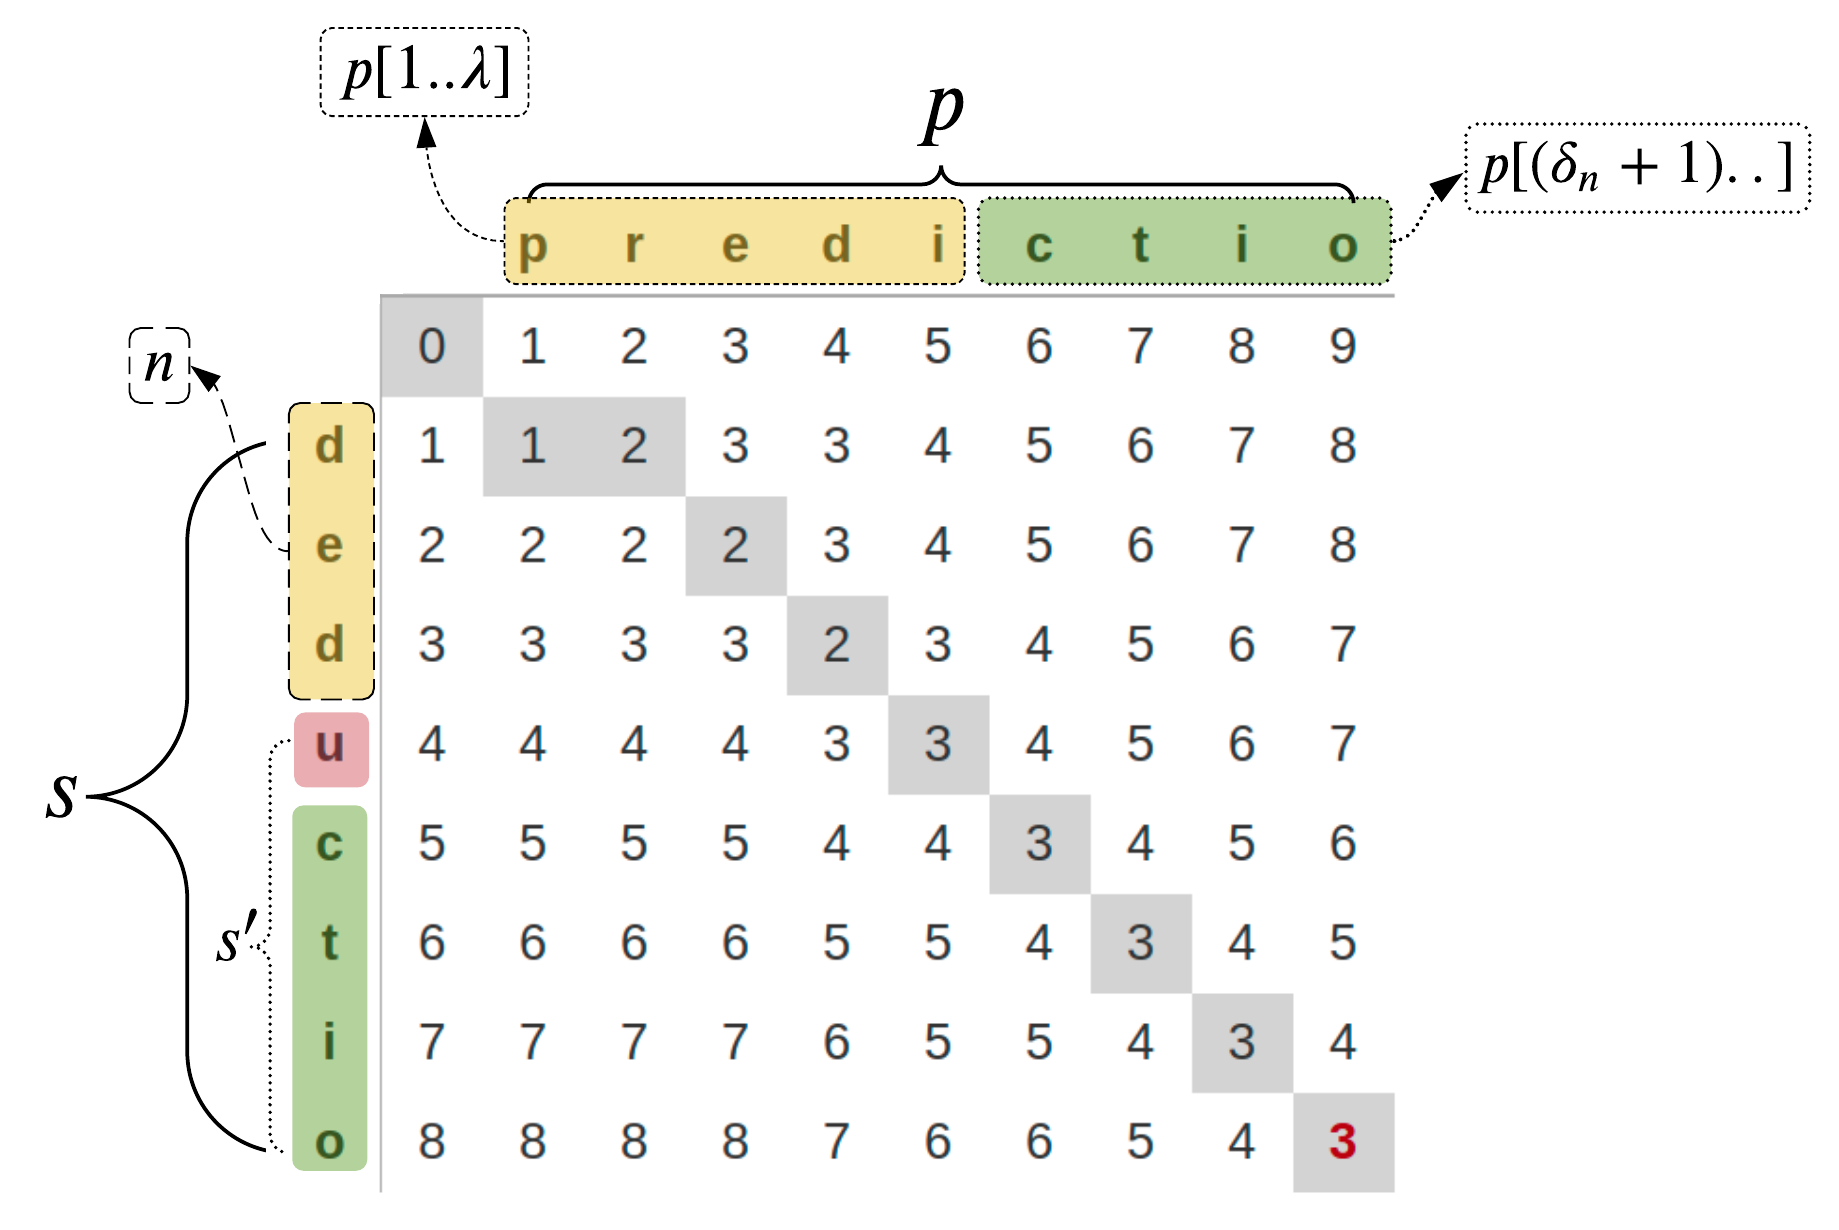
\includegraphics[width=0.94\textwidth]{figures/binary_search_counterproof.png}
    \caption{Um contra-exemplo possível que prova a imprecisão do método IP2LB, composto de uma Matriz de \textit{Levenhstein} para o cálculo de distância de edição entre $p=``predictio"$ (colunas da matriz) e a sugestão de consulta $s=``deductio"$ (linhas da matriz)}.
    \label{fig:binary_search_counterproof}
\end{figure}

A Figura~\ref{fig:binary_search_counterproof} demonstra um contra-exemplo que prova a incapacidade que o IP2LB possui de recuperar todas as sugestões de consultas similares à $p$ com até $\tau$ erros. Na figura, $\lambda = 5$, $\delta_{n}=5$, $\tau=3$. Os textos destacados em verde são, respectivamente, $p[(\delta_{n}+1)..]=``ctio"$ (o texto que é procurado pelas buscas binárias no segundo nível) e uma subcadeia $s'[2..]$ de  $s'=s[(\delta+1)..]=``uctio"$, sendo $s'[2..] = p[(\delta_{n}+1)..]$ nesse exemplo em específico. Há também os textos $``ded"$, que é o prefixo obtido a partir do caminho entre raiz da \textit{Trie} e o nó ativo de borda $n$, e $p[1..\lambda] = ``pred"$, que é o prefixo utilizado na computação de nós ativos no primeiro nível. Ambos estão coloridos em amarelo para destacar a relação entre $n$ e $p[1..\lambda]$, sendo $ed(n, p[1..\lambda] = \tau$. Além disso, há também a Matriz de \textit{Levenhstein} do cálculo de distância de edição entre $p=``predictio"$ e a sugestão de consulta $s=``deductio"$, que aliás possui o valor $3$ como podemos observar no valor da célula do canto inferior direito. Uma vez que $ed(s, p) \leq \tau$, então $s$ deve ser uma das consultas sugeridas como resposta da CATE para o prefixo de consulta $p$.

No entanto, quando o algoritmo IP2LB realiza as buscas binárias em $n$, o nó ativo de borda desse exemplo, $s$ não será incluída no conjunto de respostas para a consulta $p$ pois $p[(\delta_{n}+1)..]$, que mesmo sendo uma subcadeia de $s'$, não é encontrado nos primeiros caracteres de $s'$ como estabelecido na seção~\ref{sec:IP2LB}. Se não houvesse o caractere ``u'' (destacado em vermelho) em $s$, ou seja, se $s$ fosse $``dedctio"$, o algoritmo IP2LB consideraria $s$ como uma das sugestões válidas como resposta para a consulta. Essa falha também ocorre com outras sugestões no segundo nível do IP2LB, que por consequência não retorna alguns resultados que deveria.

Sendo assim, percebemos que não é possível aplicar a busca binária em todos os nós ativos cuja distância de edição é igual ao limiar $\tau$ sem que haja perda de resultados. Diante disso, na tentativa de resolver esse problema formulamos a hipótese de que é possível melhorar a acurácia do IP2LB restringindo a realização da busca binária para apenas alguns nós ativos de borda. Sendo $\langle n_{b}, \xi_{n_{b}}^{p[1..\lambda]}, p_{i}, \xi_{n_{b}}^{p_{i}}, \delta_{n_{b}} \rangle$ a 5-upla de um nó ativo de borda $n_b$, realizamos a busca binária nesse nó somente se $\delta_{n_{b}} = \lambda$, ou em outras palavras, se o caractere de $p[1..\lambda]$ que estava sendo processado quando $n_{b}$ foi ativado foi o $\lambda$-ésimo caractere. Essa é uma proposta de adaptação necessária para a utilização da ideia de combinar busca binária e sequencial no segundo nível, sendo uma possível resposta para a questão de pesquisa ii), apresentada na seção~\ref{sec:research-problem}. Denominamos esse método como ``IP2LRB'' (\textbf{I}C\textbf{P}AN \textbf{2}-\textit{\textbf{L}evel with \textbf{R}estricted \textbf{B}inary Search}). O algoritmo para o IP2LRB é idêntico ao Algoritmo~\ref{alg:ip2lb}, com apenas uma modificação da condição verificada na linha 6 para esta: ``$\xi_{n}^{p[1..\lambda]} = \tau \land \delta_{n} = \lambda$''.

Essa restrição faz com que a busca binária passe a ser realizada em somente $15\% \sim 40\%$ do total de nós ativos de $\Psi_{p[1..\lambda]}$, em contraste aos $75\% \sim 95\%$ do método IP2LB. O efeito disso é que o tempo de processamento de consultas do IP2LRB aproxima-se do tempo do método IP2L, porém trazendo um pouco mais de resultados que antes estavam faltando com o IP2LB. No entanto, mesmo com essa restrição o IP2LRB não consegue ter acurácia absoluta, pois ainda não traz $100\%$ dos resultados que deveria. Com isso, pensando na questão de pesquisa i) concluímos que não é possível adaptar sistemas de busca em dois níveis para tirarem proveito da busca binária no segundo nível sem que haja algum impacto na acurácia do método.
\newpage
\thispagestyle{empty}
\mbox{}
\newpage

% ---------------------
% Resultados
% ---------------------
\section{Resultados}
\label{sec:results}

O método proposto na seção~\ref{sec:metodo} foi implementado na linguagem \textit{C++} para um melhor desempenho, e também possibilitar uma comparação mais justa com os \textit{baselines}, os quais também foram todos implementados em \textit{C++}. 

\subsection{Configuração dos experimentos}
\label{sec:experiments-setup}
Nos experimentos são comparados os seguintes algoritmos:
\begin{itemize}
    \item ICAN \citep{ji2009efficient}
    \item ICPAN \citep{li2011efficient}
    \item META \citep{deng2016meta}
    \item IP2L -- Uma variação do método apresentado na seção~\ref{sec:metodo} que processa todos os nós pivô ativos com busca sequencial, sem utilizar a busca binária.
    \item IP2LB -- Método apresentado na seção~\ref{sec:metodo} na íntegra.
\end{itemize}

Os resultados de tempo processamento do META não serão considerados na exibição dos gráficos de linha, pois seus valores são muito maiores, o que dificulta a visualização dos gráficos. Além disso, todos os códigos-fonte dos \textit{baselines} são os originais utilizados pelos autores de seus respectivos artigos.

Todos os experimentos foram realizados em uma máquina de servidor com processador \textit{Intel \textsuperscript{\textregistered} Xeon E5 4617 2.90 GHz}, com \textit{64GB} de memória \textit{RAM}, tendo o \textit{Ubuntu 18.04.1 LTS} como sistema operacional. Os algoritmos foram compilados com o \textit{gcc 7.4.0}. Os experimentos aqui apresentados servem para provar o conceito do método proposto neste trabalho, mas planejamos ainda realizar um novo conjunto de experimentos mais robustos e detalhados para concluir a pesquisa.

Utilizamos uma base de dados pública denominada \textit{USADDR}, a qual é um conjunto com $10$ milhões de endereços e localizações dos Estados Unidos da América, extraídos da coleção \textit{SimpleGEO CC0}. Dessa base, os itens foram extraídos e inseridos em um único arquivo de texto no qual cada linha representa um item. Nela há um total de $10.251.121$ itens e $32.407.449$ palavras com tamanho médio igual a $6,249$ caracteres. Cada item possui uma média de $3,161$ palavras e tamanho médio médio igual a $19,757$ caracteres.

Todos os experimentos para medir o tempo de processamento foram realizados com uma média de $50$ consultas extraídas aleatoriamente da base de dados, com tamanhos variando de $3$ a $13$ (aumentando de $2$ em $2$), considerando $\tau=3$. Todas essas consultas tiveram seu terceiro caractere modificado por um novo diferente do atual, representando um erro de substituição. Para cada execução de cada algoritmo, também foi medido seu pico de memória utilizado.

\subsection{Tempo de processamento do método IP2LB}

A Tabela~\ref{tab:metodo-performance} apresenta a média de tempos (em $ms$) de processamento de consultas de prefixo $q$ utilizando o método IP2LB. A primeira coluna ``carac.'' representa os valores de $\lambda$ variando de $4$ até $10$, e as próximas colunas contêm as médias de tempo de processamento para cada tamanho $|q|$ de consulta. Para cada valor de $\lambda$ foram realizadas $50$ consultas como descrito na seção~\ref{sec:experiments-setup}, pois na prática cada valor de $\lambda$ para o método IP2LB (e IP2L) produz um modelo por si só, denominado IP2LB-$\lambda$.

\begin{table}[h]
\centering
\begin{tabular}{c|c|c|c|c|c|c|}
\cline{2-7}
 & \multicolumn{6}{c|}{\textbf{Tamanho do Prefixo Consultado}} \\ \hline
\multicolumn{1}{|c|}{\textbf{carac.}} & \textbf{|q| = 3} & \textbf{|q| = 5} & \textbf{|q| = 7} & \textbf{|q| = 9} & \textbf{|q| = 11} & \textbf{|q| = 13} \\ \hline
\multicolumn{1}{|c|}{4} & 104.414 & 225.847 & 255.190 & 262.910 & 273.861 & 263.856 \\ \hline
\multicolumn{1}{|c|}{5} & 116.767 & 58.892 & 117.848 & 117.092 & 124.004 & 129.742 \\ \hline
\multicolumn{1}{|c|}{6} & 118.174 & 67.707 & 83.576 & 85.318 & 90.690 & 92.876 \\ \hline
\multicolumn{1}{|c|}{7} & 123.378 & 71.812 & 71.817 & 79.232 & 82.692 & 85.913 \\ \hline
\multicolumn{1}{|c|}{8} & 122.283 & 74.391 & 75.281 & 78.995 & 82.135 & 84.005 \\ \hline
\multicolumn{1}{|c|}{9} & 125.307 & 76.704 & 78.162 & 77.523 & 83.250 & 83.335 \\ \hline
\multicolumn{1}{|c|}{10} & 120.886 & 77.993 & 80.702 & 79.195 & 85.414 & 119.491 \\ \hline
\end{tabular}
\caption{Tempos de processamento em $ms$ para o método IP2LB variando o tamanho do prefixo de consulta $q$ e variando também o $\lambda$ (coluna ``carac.''), a altura máxima para a \textit{Trie}.}
\label{tab:metodo-performance}
\end{table}

Na Figura~\ref{fig:varying-usaddr-tau-3} estão representados os resultados da Tabela~\ref{tab:metodo-performance}. Há $7$ curvas (uma para cada valor de $\lambda$) de tempo de processamento em função do tamanho da consulta, para o método IP2LB variando o tamanho do prefixo de consulta $q$ e variando também o $\lambda$, a altura máxima para a \textit{Trie}. 

\begin{figure}[ht!]
    \centering
    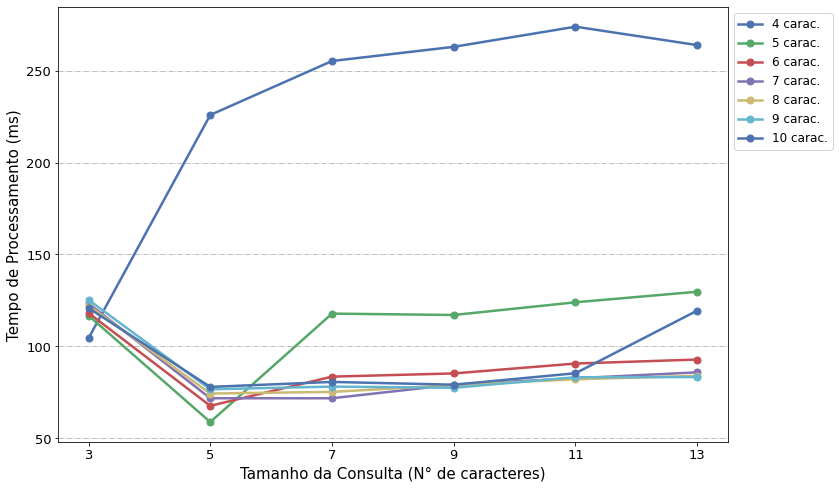
\includegraphics[width=0.95\textwidth]{figures/varying_trie_prefix_method_IP2LB_dataset_usaddr_tau_3.png}
    \caption{Curvas de tempo de processamento em $ms$ para o método IP2LB variando o tamanho do prefixo de consulta $q$ e variando também o $\lambda$, a altura máxima para a \textit{Trie}.}
    \label{fig:varying-usaddr-tau-3}
\end{figure}

É esperado que, quanto maior for o valor de $\lambda$, menor será o tempo de processamento. Essa tendência pode ser observado no gráfico da Figura~\ref{fig:varying-usaddr-tau-3}. No entanto, para $\lambda = 4$ a sua curva de tempos se distancia bastante das demais. Isso provavelmente ocorre porque, dada a natureza do algoritmo ICPAN, no término do primeiro nível há uma grande quantidade de nós ativos quando se indexa somente os $4$ primeiros caracteres na \textit{Trie} (mesmo com sua otimização de poda de nós ativos redundantes).

\subsection{Uso de memória do método IP2LB}

A Tabela~\ref{tab:memory-usage-usaddr-tau-3} exibe a quantidade memória utilizada pelo método IP2LB (segunda coluna) para cada valor de $\lambda$ (primeira coluna).

\begin{table}[!ht]
\centering
\begin{tabular}{|c|c|}
\hline
\textbf{carac.} & \textbf{Memória Utilizada (MB)} \\ \hline
4 & 1378.490 \\ \hline
5 & 1408.363 \\ \hline
6 & 1528.575 \\ \hline
7 & 1749.214 \\ \hline
8 & 2075.432 \\ \hline
9 & 2520.842 \\ \hline
10 & 3078.759 \\ \hline
\end{tabular}
\caption{Quantidades de memória em \textit{MegaBytes} utilizada para cada valor de $\lambda$ no método IP2LB.}
\label{tab:memory-usage-usaddr-tau-3}
\end{table}

A Figura~\ref{fig:memory-usage-usaddr-tau-3} representa os dados da Tabela~\ref{tab:memory-usage-usaddr-tau-3}, contendo uma curva da quantidade de memória utilizada pelo método IP2LB em função do valor de $\lambda$.

\begin{figure}[!ht]
    \centering
    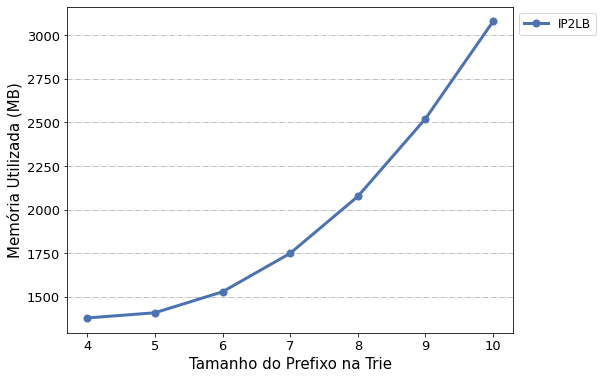
\includegraphics[width=0.95\textwidth]{figures/memory_usage_IP2LB_dataset_usaddr_tau_3.png}
    \caption{Curva de quantidades de memória em \textit{MegaBytes} utilizada para cada valor de $\lambda$ no método IP2LB.}
    \label{fig:memory-usage-usaddr-tau-3}
\end{figure}

É possível observar um padrão exponencial no consumo de memória à medida que a altura máxima permitida para a \textit{Trie} aumenta. Isso acontece pois a função do número máximo de nós a cada nível de uma árvore $M-\text{á}ria$ como a \textit{Trie} \citep{Knuth:1998} é de fato exponencial com base no tamanho do alfabeto $\Sigma$ considerado. Quanto menos prefixos em comum houver entre os itens indexados, mais o padrão de uso exponencial de memória será atingido.

\subsection{Tempo de processamento de todos os métodos}

A Tabela~\ref{tab:performance-usaddr-tau-3} apresenta as médias de tempo de processamento (em $ms$) para cada método, considerando $\lambda=6$ para IP2LB e o IP2L. Tal valor de $\lambda$ foi escolhido com a intenção de melhor otimizar a relação desempenho/consumo de memória para ambos os métodos. 

\begin{table}[ht]
\centering
\begin{tabular}{c|c|c|c|c|c|c|}
\cline{2-7}
 & \multicolumn{6}{c|}{\textbf{Tamanho da Consulta}} \\ \hline
\multicolumn{1}{|c|}{\textbf{alg.}} & \textbf{|q| = 3} & \textbf{|q| = 5} & \textbf{|q| = 7} & \textbf{|q| = 9} & \textbf{|q| = 11} & \textbf{|q| = 13} \\ \hline
\multicolumn{1}{|c|}{IP2LB-6} & 118.174 & 67.707 & 83.576 & 85.318 & 90.690 & 92.876 \\ \hline
\multicolumn{1}{|c|}{IP2L-6} & 119.540 & 67.749 & 125.885 & 148.891 & 155.325 & 158.376 \\ \hline
\multicolumn{1}{|c|}{ICPAN} & 152.106 & 118.598 & 123.010 & 125.072 & 130.454 & 134.613 \\ \hline
\multicolumn{1}{|c|}{ICAN} & 198.942 & 176.930 & 200.260 & 201.083 & 209.302 & 200.332 \\ \hline
\multicolumn{1}{|c|}{META} & 3180.390 & 5458.480 & 5583.350 & 5794.830 & 6021.520 & 6006.690 \\ \hline
\end{tabular}
\caption{Tempos de processamento em $ms$ dos métodos, considerando $\lambda = 6$ para os métodos IP2LB e IP2L.}
\label{tab:performance-usaddr-tau-3}
\end{table}

A Figura~\ref{tab:performance-usaddr-tau-3} contém uma curva de tempo de processamento em função do tamanho do prefixo de consulta as médias de tempo de processamento (em $ms$) para cada método, considerando $\lambda=6$ para IP2LB e o IP2L.

\begin{figure}[ht]
    \centering
    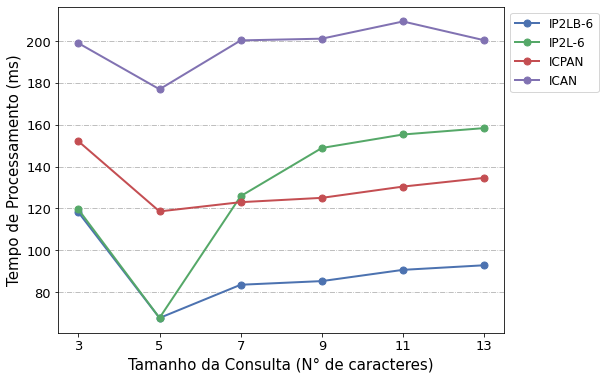
\includegraphics[width=0.9\textwidth]{figures/performance_baselines_dataset_usaddr_tau_3.png}
    \caption{Curvas de tempo de processamento em $ms$ dos métodos, considerando $\lambda = 6$ para os métodos IP2LB e IP2L.}
    \label{fig:performance-usaddr-tau-3}
\end{figure}

O método com melhor desempenho foi o IP2LB-6. Também é possível observar que o método IP2L, sem a busca binária no segundo nível, atinge tempos de processamento maiores que o ICPAN para consultas de tamanho maior que $7$, enquanto no mesmo cenário o método IP2LB-6 mantém-se aproximadamente $40\%$ mais rápido que o ICPAN. Além disso, o formato das curvas dos métodos ICPAN e IP2LB apresentam um formato similar. Isso demonstra que a busca binária nos nós ativos de borda do segundo nível consegue ``estabilizá-lo'' de forma que o desempenho da estrutura completa mantém-se, no mínimo, semelhante ao do algoritmo utilizado no primeiro nível.

\subsection{Uso de memória de todos os métodos}

A Tabela~\ref{tab:memory-usage-usaddr-tau-3} apresenta a média do consumo de memória (em \textit{MegaBytes}) para cada método, considerando $\lambda=6$ para IP2LB e o IP2L.

A Figura~\ref{fig:memory-usage-usaddr-tau-3} representa os resultados da Tabela~\ref{tab:memory-usage-usaddr-tau-3} em forma de gráficos de barras, havendo uma barra para método, com média de seu consumo de memória (em \textit{MegaBytes}).

O uso da estrutura de busca em dois níveis resultou em uma redução de $80\%$ do uso de memória aproximadamente, considerando o IP2LB e o ICPAN, por exemplo.

\newpage
\begin{table}[h]
\centering
\begin{tabular}{|c|c|}
\hline
\textbf{alg.} & \textbf{Memória Utilizada (MB)} \\ \hline
IP2LB-6 & 1528.575 \\ \hline
IP2L-6 & 1528.487 \\ \hline
ICPAN & 9101.487 \\ \hline
ICAN & 9125.932 \\ \hline
META & 7618.745 \\ \hline
\end{tabular}
\caption{Quantidades de memória em \textit{MegaBytes} utilizada por cada método, considerando $\lambda = 6$ para os métodos IP2LB e IP2L.}
\label{tab:memory-usage-baselines-usaddr-tau-3}
\end{table}

\begin{figure}[h]
    \centering
    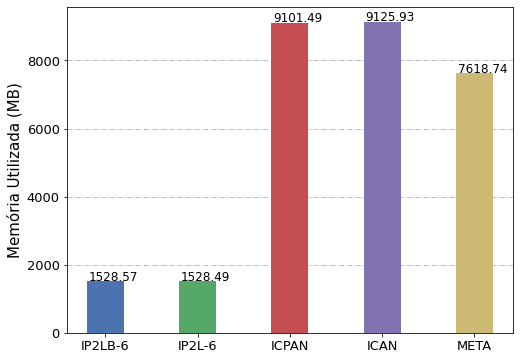
\includegraphics[width=0.8\textwidth]{figures/memory_usage_baselines_dataset_usaddr_tau_3.png}
    \caption{Gráfico de barras para as quantidades de memória em \textit{MegaBytes} utilizada por cada método, considerando $\lambda = 6$ para os métodos IP2LB e IP2L.}
    \label{fig:memory-usage-baselines-usaddr-tau-3}
\end{figure} 

\cleardoublepage

\newpage
\thispagestyle{empty}
\mbox{}
\newpage

% ---------------------
% Conclusão
% ---------------------
\section{Conclusão}
\label{sec:conclusion}

Os experimentos preliminares realizados mostram que a estratégia de dois níveis com a combinação de busca sequencial e binária no segundo nível não só permitiram uma significante economia de memória, quanto mantiveram a eficiência no processamento das consultas. O uso da busca binária torna o segundo nível muito mais estável, pois reduz a complexidade algorítmica de grande parte do processamento realizado no segundo nível.

O BEVA é o atual estado da arte, apresentando tempo de processamento $11$ vezes mais rápido que o ICPAN \citep{zhou2016beva}, e utilizá-lo no primeiro nível juntamente com a combinação de buscas no segundo nível é uma ideia que apresenta possibilidades de ótimos resultados.



% % ----------------------------------------------------------
% % ELEMENTOS PÓS-TEXTUAIS
% % ----------------------------------------------------------
% \postextual


% % ----------------------------------------------------------
% % Referências bibliográficas
% % ----------------------------------------------------------
\newpage
 \bibliography{referencias}

% ----------------------------------------------------------
% Glossário
% ----------------------------------------------------------
%
% Consulte o manual da classe abntex2 para orientações sobre o glossário.
%
%\glossary

% ----------------------------------------------------------
% Apêndices
% ----------------------------------------------------------

% ---
% Inicia os apêndices
% ---
% \begin{apendicesenv}

% % Imprime uma página indicando o início dos apêndices
% \partapendices

% % ----------------------------------------------------------
% \chapter{Quisque libero justo}
% % ----------------------------------------------------------

% \lipsum[50]

% % ----------------------------------------------------------
% \chapter{Nullam elementum urna vel imperdiet sodales elit ipsum pharetra ligula
% ac pretium ante justo a nulla curabitur tristique arcu eu metus}
% % ----------------------------------------------------------
% \lipsum[55-57]

% \end{apendicesenv}
% ---


% ----------------------------------------------------------
% Anexos
% ----------------------------------------------------------

% ---
% Inicia os anexos
% ---
% \begin{anexosenv}

% % Imprime uma página indicando o início dos anexos
% \partanexos

% % ---
% \chapter{Morbi ultrices rutrum lorem.}
% % ---
% \lipsum[30]

% % ---
% \chapter{Cras non urna sed feugiat cum sociis natoque penatibus et magnis dis
% parturient montes nascetur ridiculus mus}
% % ---

% \lipsum[31]

% % ---
% \chapter{Fusce facilisis lacinia dui}
% % ---

% \lipsum[32]

% \end{anexosenv}

%---------------------------------------------------------------------
% INDICE REMISSIVO
%---------------------------------------------------------------------

\printindex

\end{document}
